\chapter{基于双向跨模态实体重构的神经机器翻译}

% 改进:
%    删去的:解码器、短语重构、目标端重构
%    增加的:文本->重构,句子级语义融合
%上一章提出了一种基于明确的图文实体替换的文本重构方法,该方法能够利用图片中视觉目标所携带的信息提升实体词的翻译准确率。虽然为整体的翻译准确率带来了一定的提升,但其一方面采用的是图片到文本单向的重构方法,相关研究表明由文本生成图像的过程也能够提升神经机器翻译的翻译质量;另一方面,原文到原文的生成过程将大量的训练资源浪费在将源端的单词复制到目标端,仅做到了将文本上下文信息融合到视觉目标对应的单词中,却难以将视觉信息融合到文本上下文中。
上一章提出了一种基于明确的图文实体替换的文本重构方法,该方法能够利用图片中视觉目标所携带的信息提升实体词的翻译准确率。虽然为整体的翻译准确率带来了一定的提升,但其一方面仅采用了图片到文本单向的重构方法,另一方面,原文到原文的生成过程将大量的训练资源浪费在将源端的单词复制到目标端,难以将视觉信息融合到文本上下文中。
%虽然有效,但模型也在学习复制过程,抛弃了图片信息与文本信息的相互融合。
为解决以上问题,本章提出了一种基于双向跨模态实体重构的神经机器翻译方法,并在训练中增加了将图片中视觉目标信息与文本上下文融合的任务。所提方法分为视觉目标到词的文本实体重构,文本到视觉目标的视觉实体重构,以及文本上下文与视觉目标组合到非实体词的文本非实体重构三个子任务。其能够更加充分地利用图片中所包含的视觉信息,从而提升神经机器翻译模型的翻译质量。
% 实验结果
实验结果展示了所提方法进一步提升翻译质量的能力,进一步的分析展示了方法的有效性。
\section{引言}
%第一部分应该讲一些能够引入sec3不足的方面,即如何更充分的利用视觉信息
%可以从预训练模型的角度去分析仅采用一种task的方式的不足
%本章可以强调多任务的“多”,上一章更应该是双任务
传统的融合图片信息的神经机器翻译方法采取将图片作为额外输入的方式,从而使翻译模型在编码或解码阶段尽可能地利用其所携带的视觉信息。然而这类方法很难达到理想的效果,图片作为外源信息难以被直接利用。相比之下,采用多任务学习的方式将外源信息融合到神经机器翻译中成为一种可行的方案\cite{49_wang-zhang-2022-addressing,50_kang_zong_2022}。


%第二部分从上一章做了哪些具体内容,详细分析其不足,例如为何重构文本存在资源浪费,为何只有文本上下文到视觉目标的融合。
上一章提出的跨模态文本重构方法采用了文本重构任务,尝试在跨模态编码和文本解码生成两个阶段将图片中的视觉目标信息融合到词的表示中,并为模型的翻译质量带来了提升。但该方法仍存在着一定的不足和需要改进的地方:一是所采用的重构方案是单向的,仅考虑了图片到文本方向,文献\cite{37_elliott-kadar-2017-imagination}表明文本到图像的生成同样可以提升模型的翻译质量,因此存在未充分利用视觉信息的可能;二是原文到原文的生成训练,很容易使模型的编码-解码过程收敛为“复制-粘贴”过程,这种极端情况下除了视觉目标对应位置可以从图片以及上下文中获取信息用于生成目标单词,其它词在编码和解码过程中难以融合信息,只是将源语言的词复制并粘贴到目标端的对应位置,使整个重构模型的训练流程大量地浪费在这种“复制-粘贴”过程中。
尽管模型的实际表现并未如此不堪,但以上的分析也说明了方法存在的改进空间。

%如何解决上面的不足:双向重构(文到图的重构会带来哪些作用),文本非实体重构(为何将视觉信息融合到文本中有效果)(这两个问题需要在实验中体现)
为了解决以上问题,本章提出一种跨模态实体重构(cross-modal entity reconstruction,CER)方法用于帮助神经机器翻译提升译文的质量。该方法为了更加充分地将图片中的视觉目标信息融合到实体词的表示中,采取了图片与文本两个模态之间的双向重构策略,实现显式的跨模态信息融合。并且为了进一步提升图片信息的作用,将图片信息与文本上下文信息融合,采用了非实体的重构策略,实现隐式的跨模态信息融合。将显式方法与隐式方法融合到同一个模型中,实现对翻译模型的更进一步的增强。
具体地,CER方法分为三个子任务:
文本实体重构任务延续了上一章文本重构任务利用视觉目标与文本上下文实现重构的策略,区别在于文本实体重构任务省去了非实体词的生成过程,即只重构文本中的实体词;
视觉实体重构任务负责从文本上下文与文本实体中所提供的文本模态信息重构视觉目标实体,区别于重构完整图片的方案,视觉实体重构以更细粒度更精确的方式进行文本到图像的生成任务;
文本非实体重构任务采用部分文本上下文信息与视觉实体的组合,重构文本上下文中非实体词的部分,这样能够使图片中的视觉目标信息作用到文本的表示学习过程中,区别于上一章的文本重构方法也重构了文本非实体,本章在进行文本非实体重构时需要将源端的对应非实体信息通过掩码的方式去除,确保重构过程不是简单地从源端复制信息。
CER-NMT是结合了跨模态实体重构和非实体重构的神经机器翻译方法。在CER-NMT中,翻译任务作为主任务与CER方法的三个子任务通过多任务训练的方式相结合,从而实现对模型翻译准确率的提升。

%贡献:实体级图片重构,显式方法与隐式方法的融合,
本章主要贡献如下:

(1)本章提出了一种基于双向跨模态实体重构的神经机器翻译方法。在文本重构任务的基础上,增加了视觉实体重构和文本非实体重构两个任务,使图片中的视觉目标信息能够更充分的分别融合到句子中的文本实体与文本上下文中,最终通过多任务学习的方式增强翻译模型的表示能力,达到提升译文质量的目的。
%使得在文本的表示学习过程中图片中的视觉目标信息能够更充分地融合到

(2)本章所提方法结合了显式与隐式两种跨模态信息融合方法。文本实体重构与视觉实体重构均采用了显式跨模态实体信息融合方法,即图片信息具有明确的作用目标。文本非实体重构采用了视觉信息与文本上下文信息,因为非实体词与视觉目标没有直接的对应关系,因此视觉信息的作用目标不明确,属于隐式跨模态信息融合方法。通过结合两类方法实现对翻译模型的进一步的增强。

(3)本章所提方法使模型的翻译质量得到了进一步的提升。在对实验结果的分析中发现,CER方法能够提升模型的翻译忠实度,使翻译过程更忠于原文所提供的实体词的信息。在更进一步针对词频的翻译准确率的统计中发现,实体重构方法能够有效提升主要分布于低频词的实体词的翻译准确率,非实体重构方法对非实体词也有一定的相似效果。
% 应该强调一下多粒度跨模态信息融合方法,一个明确的粒度是实体机双向融合,另一个是句子级跨模态信息融合
\section{相关工作}
% 文本到图片的翻译

% 多任务nlp,最好是翻译

% 预训练模型:文本、多模态


% 应该侧重图片重建相关的方法,大概也就3个工作(imagination,Adversarial reconstruction for Multi-modal Machine Translation,

\section{方法描述}

\subsection{图文实体}
\label{sec:4_entities}
\begin{figure}[!htbp]
    \centering
    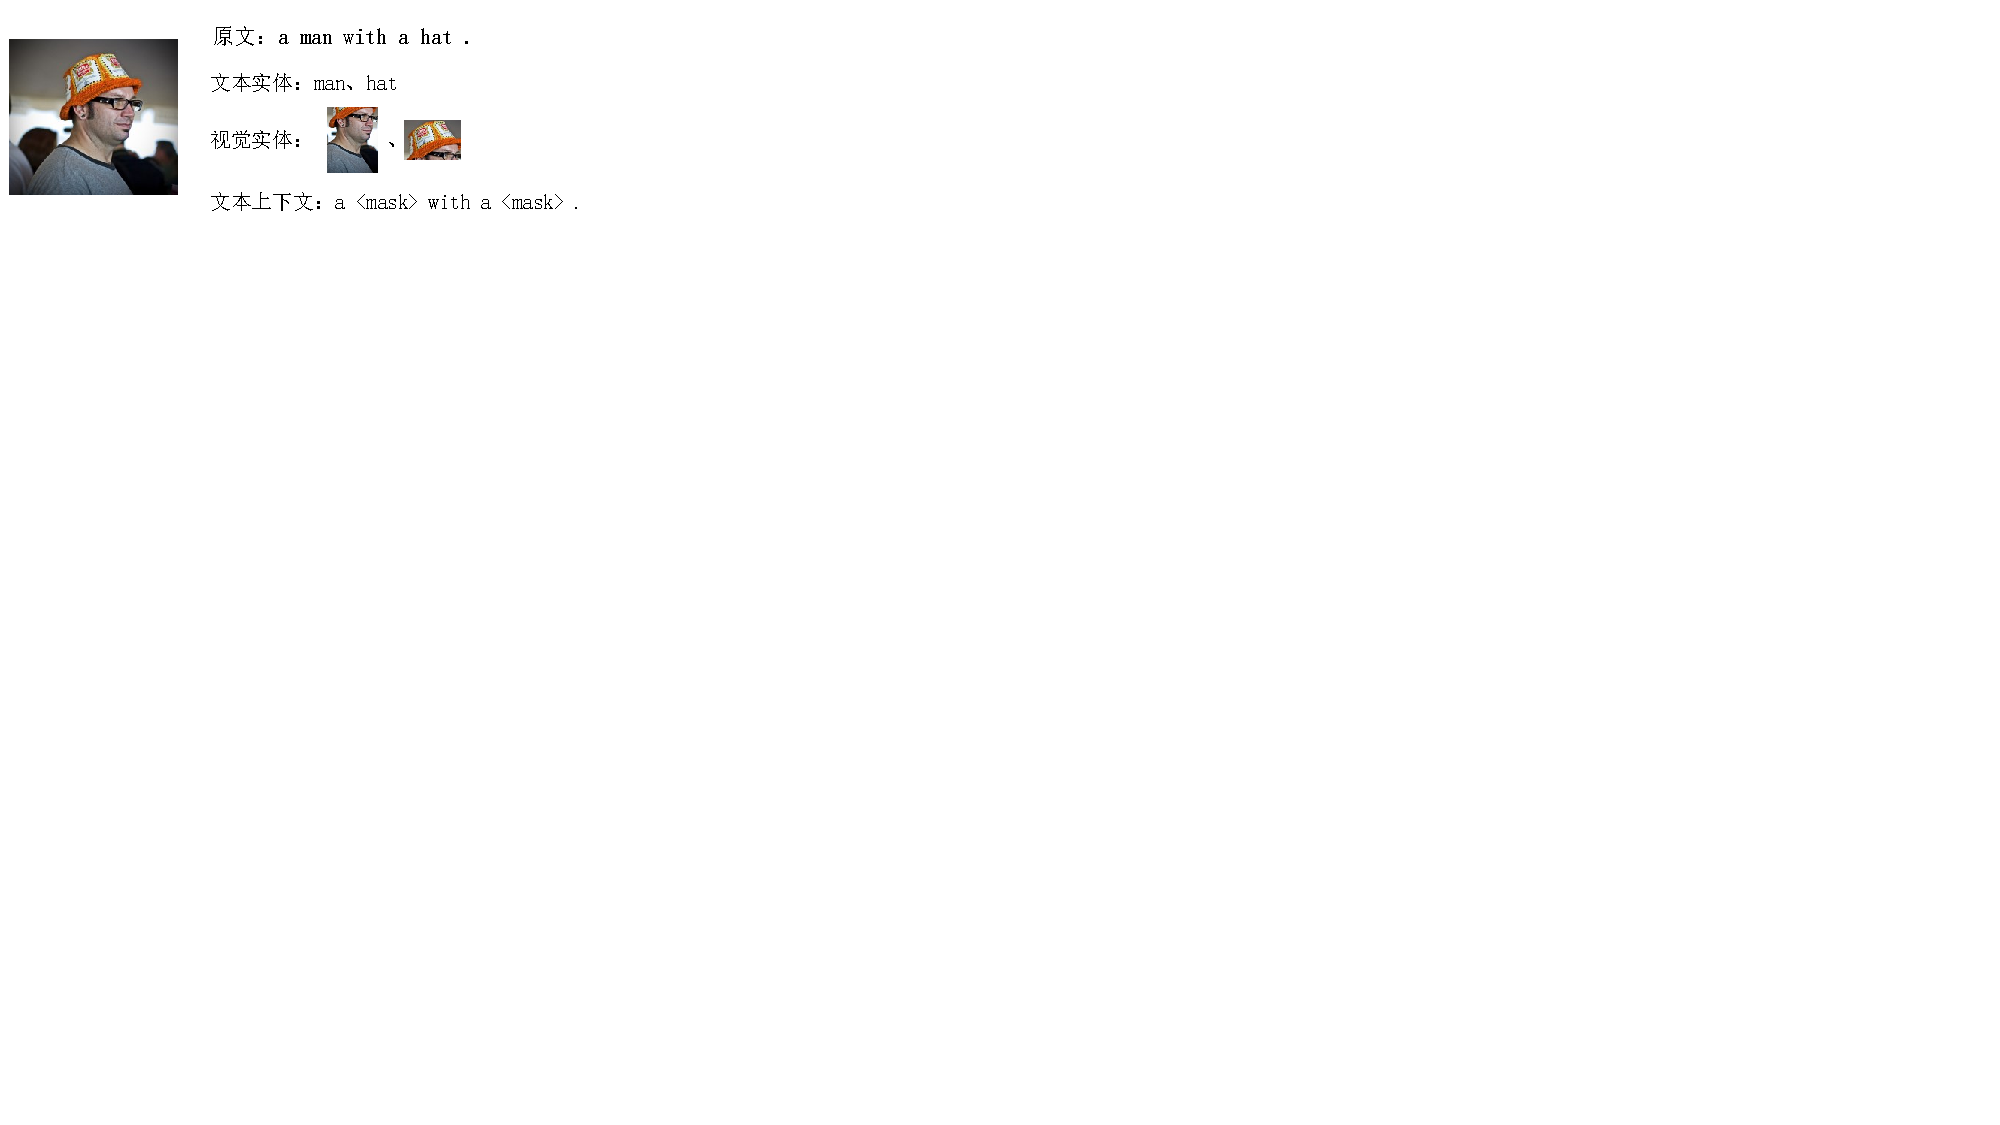
\includegraphics{Img/fig_4_definations.pdf}
    \bicaption{图文实体}{Visual entities and textual entities}
    \label{fig:4_definations}
\end{figure}
为了更方便地对本章所提的CER方法进行介绍,首先需要对CER方法作用到的图片视觉目标和文本中的作用目标进行更恰当的定义:

(1){\sffamily 文本实体:}输入的源语言句子$X=\{t_1,t_2,\cdots,t_N\}$中,在对应图片有对应视觉目标的名词$t_a,t_b,\cdots$为文本实体(textual entity),$T=\{t_a,t_b,\cdots\}$为它们的集合。如图\ref{fig:4_definations}所示,名词“man”和“hat”在图片中均有与其对应的视觉目标,因此符合文本实体的定义。从该定义同样可知,文本实体与上一章\ref{sec:3_entity_replacement}小节所介绍的词实体本质上是相同的。本章不再将名词短语划为实体范畴进行考虑,只针对名词融合视觉信息。

(2){\sffamily 视觉实体:}文本实体在对应图片$I$中的对应视觉目标${e_a,e_b,\cdots}$为视觉实体(visual entity),$E=\{e_a,e_b,\cdots\}$为它们的集合。图\ref{fig:4_definations}中的“男人”和“帽子”分别是名词实体“man”和“hat”在图片中对应的视觉目标,因此是视觉实体。

(3){\sffamily 文本非实体:}在源语言句子中,所有非文本实体的单词均可称为文本非实体(textual none-entity)。$\tilde{X}=X-T$代表它们的集合、文本上下文或退化文本。例如图\ref{fig:4_definations}中,文本上下文中除“<mask>”外均为文本非实体。

%\subsection{跨模态编码}
%\label{sec:4_cross_modal_encoding}
%\begin{figure}[!htbp]
    \centering
    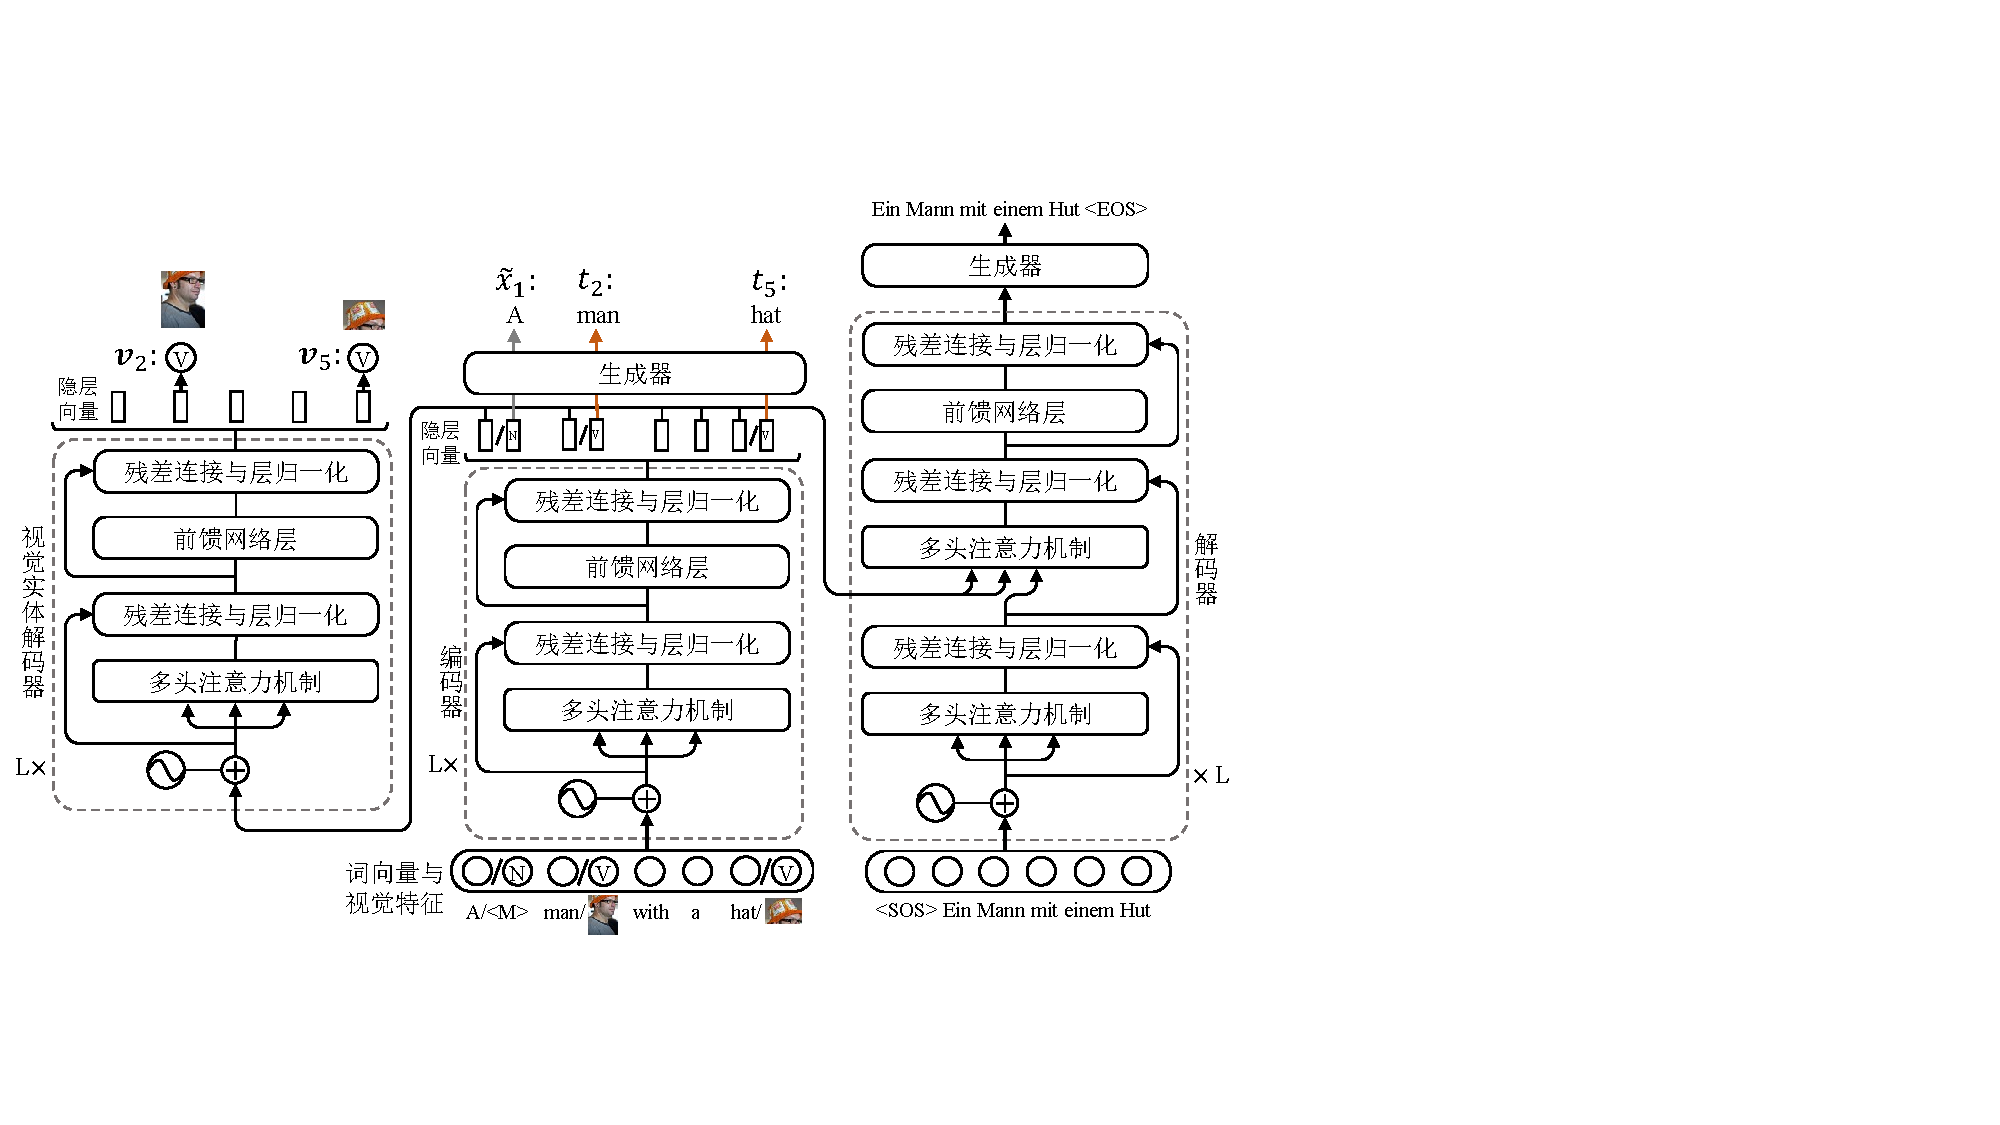
\includegraphics[scale=0.5]{Img/fig_4_model.pdf}
    \bicaption{结合跨模态实体重构方法的神经机器翻译}{NMT model framework combined with CER}
    \label{fig:4_model}
\end{figure}
%图\ref{fig:4_model}展示了CER模型与NMT模型相融合的简化过程,其中包含了视觉实体解码器、跨模态编码器以及翻译解码器三个主要组成部分。其中最核心的跨模态编码器负责在实体重构之前将视觉信息与文本信息编码融合。所编码的信息包含着实体重构主要依赖的三部分:

%\begin{itemize}
%\item
%\begin{figure}[!htbp]
    \centering
    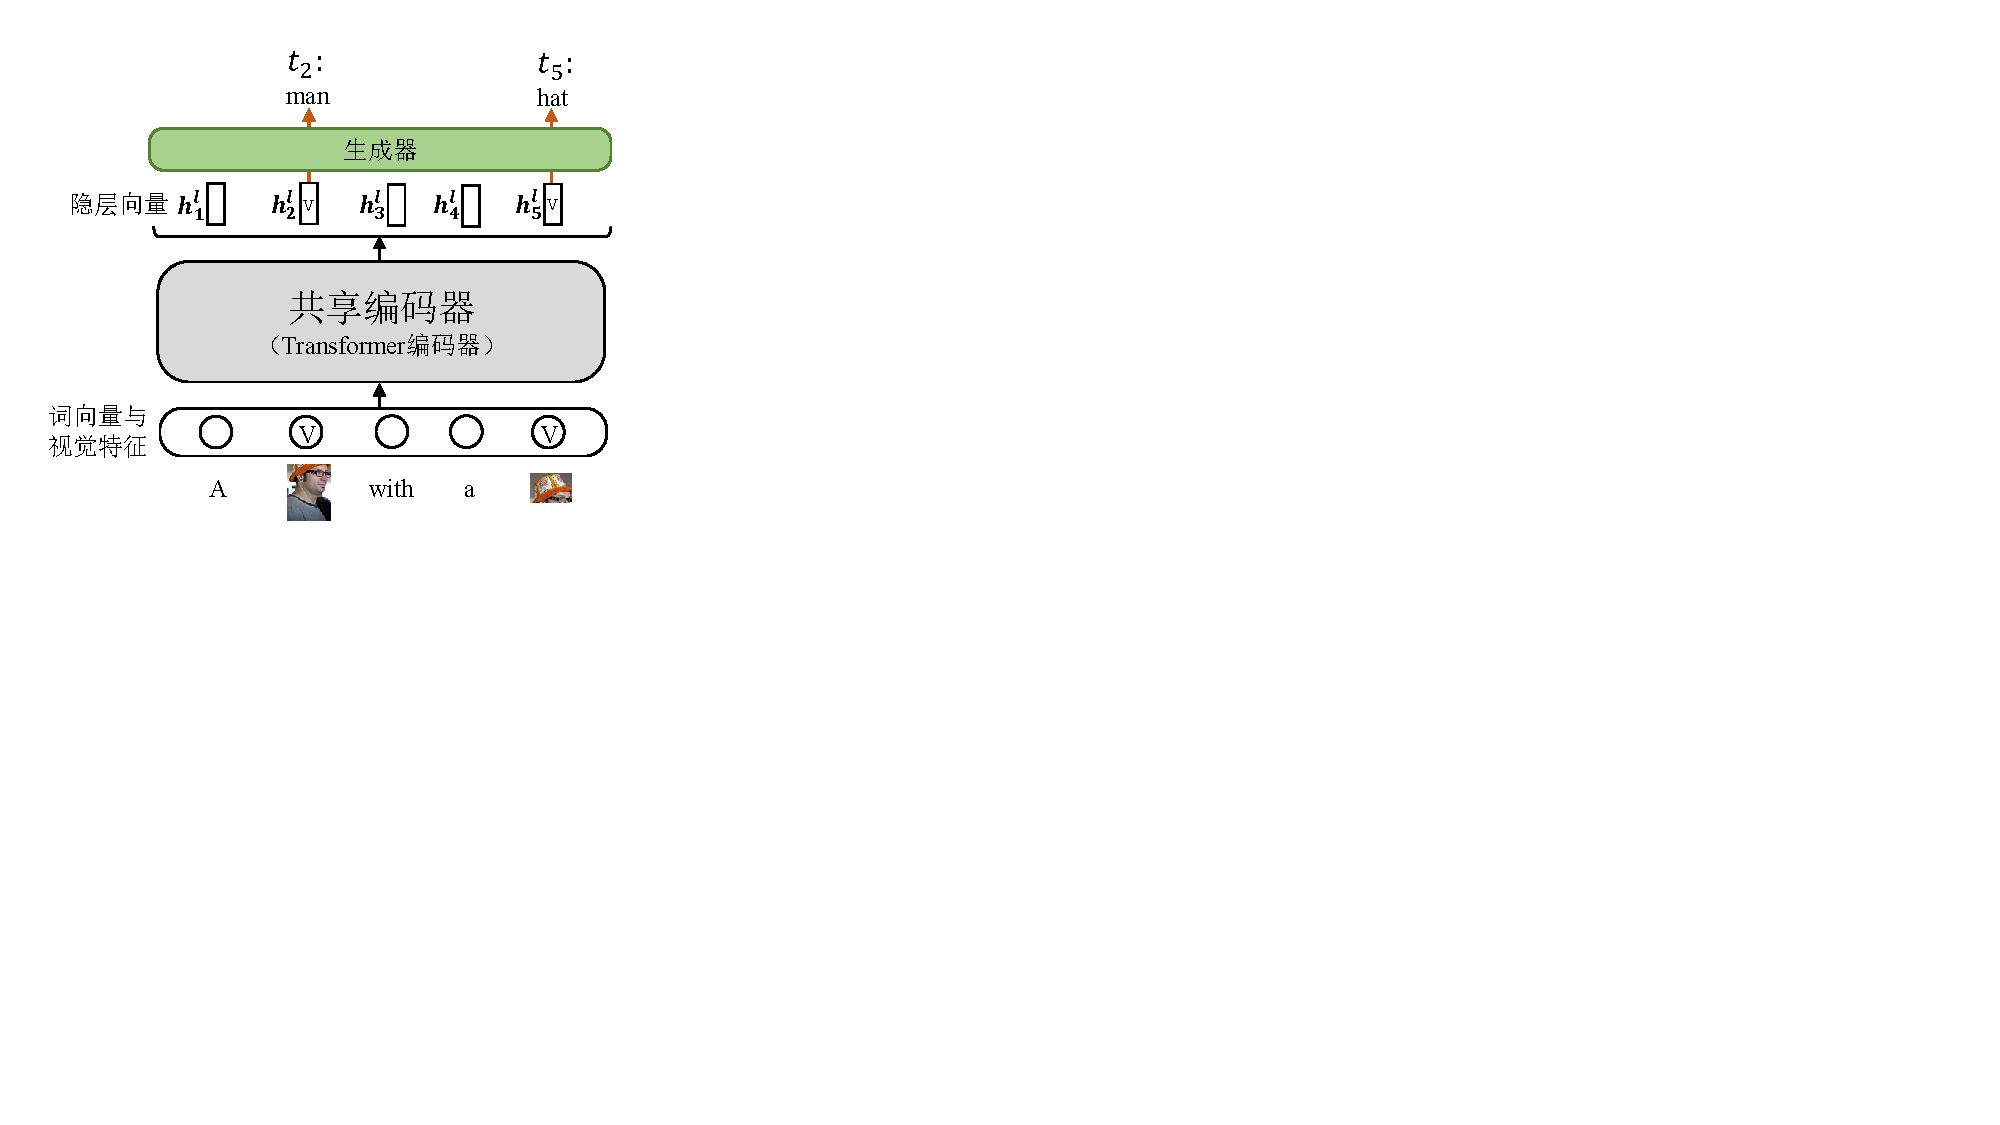
\includegraphics[scale=0.6]{Img/fig_4_ter.pdf}
    \bicaption{文本实体重构}{Textual entity reconstruction}
    \label{fig:4_ter}
\end{figure}
%(1){\sffamily 跨模态实体:}其中实体重构主要依赖于跨模态实体所提供的具体信息。如图【】所示,文本实体$t_1$的重构主要依赖于视觉实体$e_1$,视觉实体$e_1$的重构也主要依赖于文本实体$t_1$。

%\item
%(2){\sffamily 文本上下文:}本文所用文本上下文为经过退化的文本$\tilde{X}$。例如图【】中进行实体重构时,文本上下文为“A <M> with a <M>”,其中“<M>”代表将实体词所对应的位置删除并保留该位置空缺。文本上下文与跨模态实体共同组成文本的完整语义。在进行视觉实体重构时,模型的输入由文本上下文和文本实体共同组成,即原文本$X$。在进行文本实体重构时,模型的输入是文本上下文和视觉实体所组成的多模态混合序列$Z$。在进行文本非实体的重构时,模型的输入同样是多模态混合序列,但是需要将待重构的非实体词利用掩码词“<M>”替换掉,形成$\tilde{Z}$。跨模态实体与文本上下文组合重构实体的方式,既能保证重构实体时具备充足的语义信息,又能充分利用到自注意力机制的特性使实体与文本上下文建立良好的语义关系。

%\item
%(3){\sffamily 实体对齐关系:}为了避免让模型完成较为困难的跨模态实体关系对齐,本文采用直接替换对应位置向量表示的方式。例如图2中重构文本实体$t_1$时,将输入序列中的对应位置直接替换为视觉实体的向量表示${\boldsymbol{e}_1}$。

\subsection{跨模态实体重构}
\label{sec:4_cer}
\begin{figure}[!htbp]
    \centering
    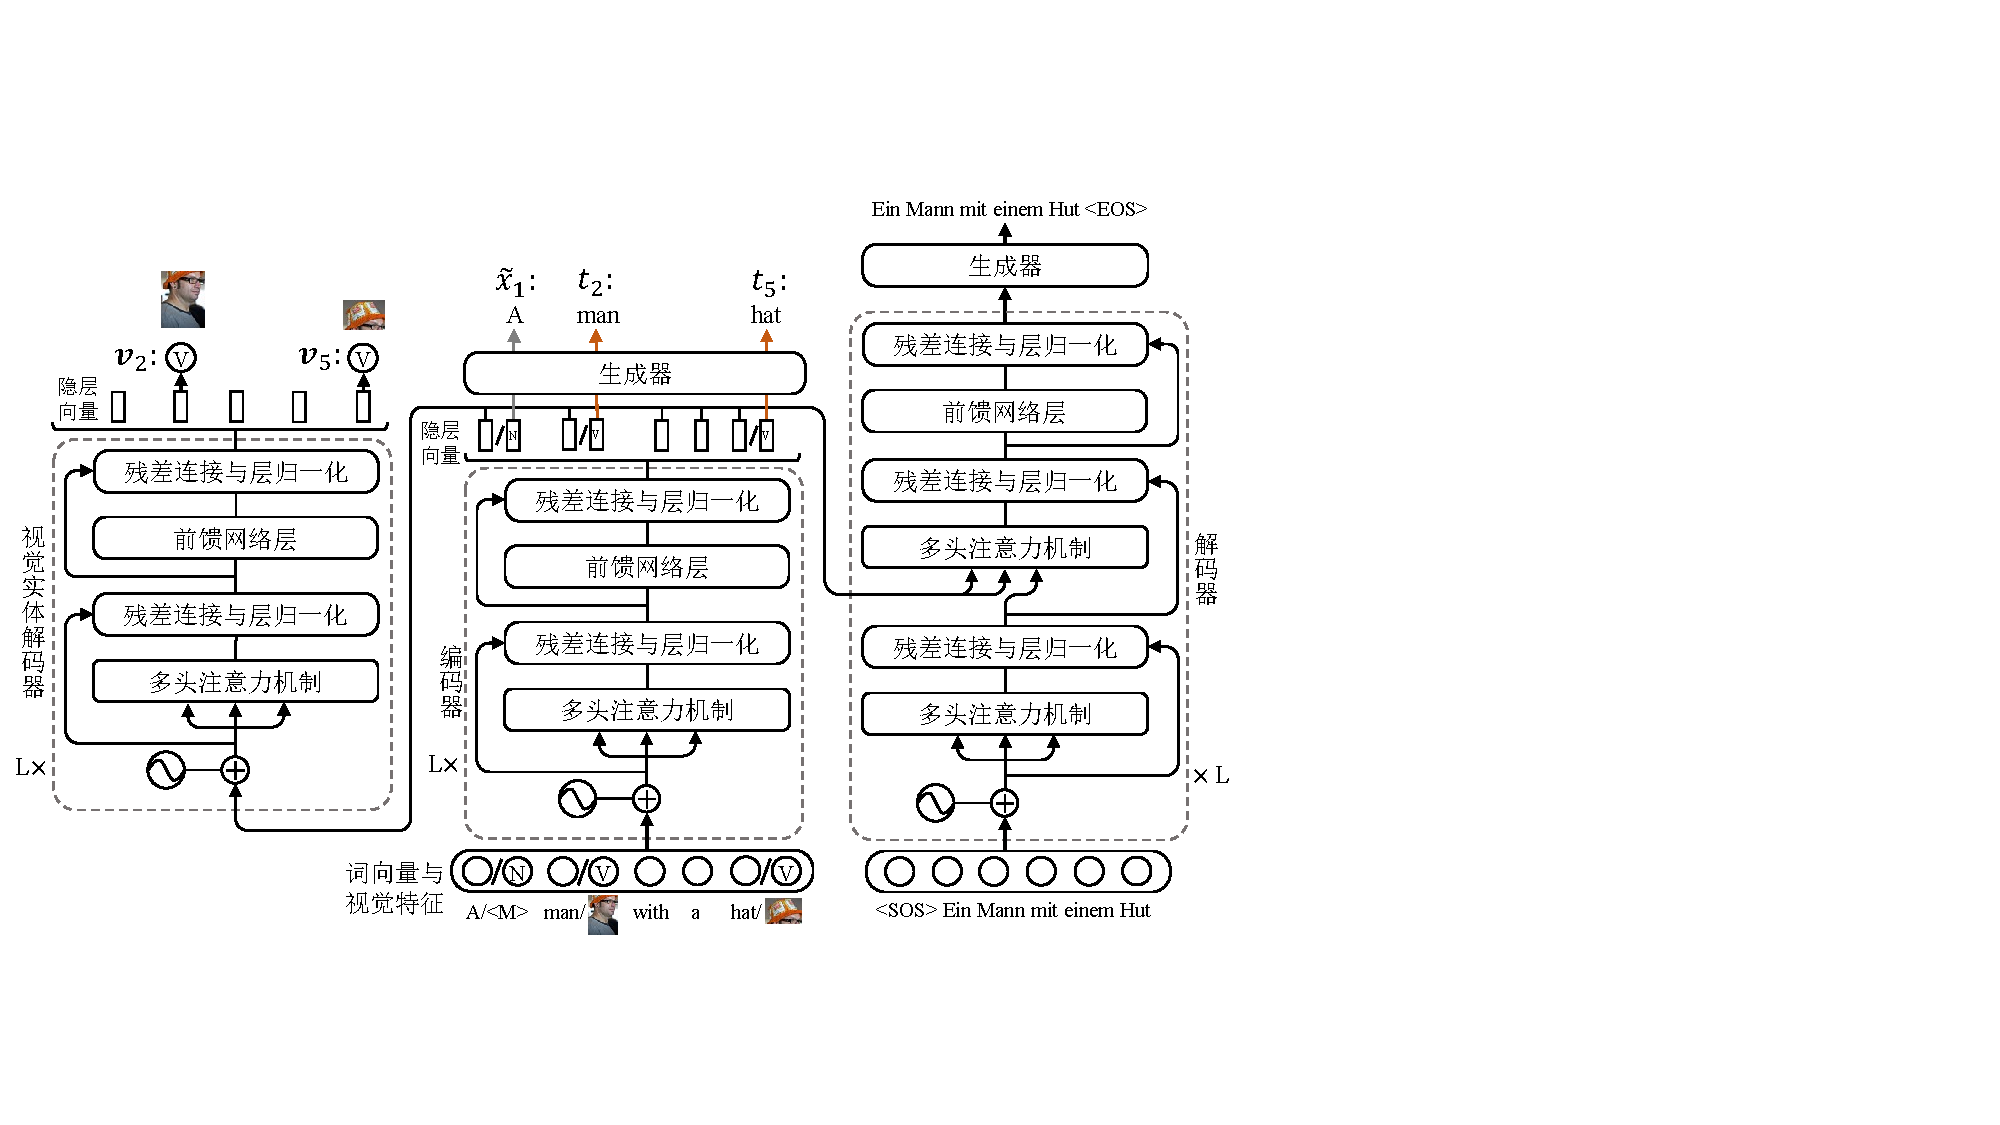
\includegraphics[scale=0.5]{Img/fig_4_model.pdf}
    \bicaption{结合跨模态实体重构方法的神经机器翻译}{NMT model framework combined with CER}
    \label{fig:4_model}
\end{figure}
图\ref{fig:4_model}展示了CER模型与NMT模型相融合的简化过程,其中包含了视觉实体解码器、跨模态编码器以及翻译解码器三个主要组成部分。其中最核心的跨模态编码器负责在实体重构之前将视觉信息与文本信息编码融合。解码器仅用于主任务翻译的目标文本解码。视觉实体解码器负责将跨模态编码器编码后的状态解码到视觉目标所代表的视觉语义空间,而其结构与编码器相同均为$L$层Transformer编码器。为了更详细地介绍CER方法是如何工作的,以及如何与神经机器翻译相结合,本节将CER方法分为:文本实体重构、视觉实体重构以及文本非实体重构三个子任务进行详细的介绍。

{\sffamily 文本实体重构}

\begin{figure}[!htbp]
    \centering
    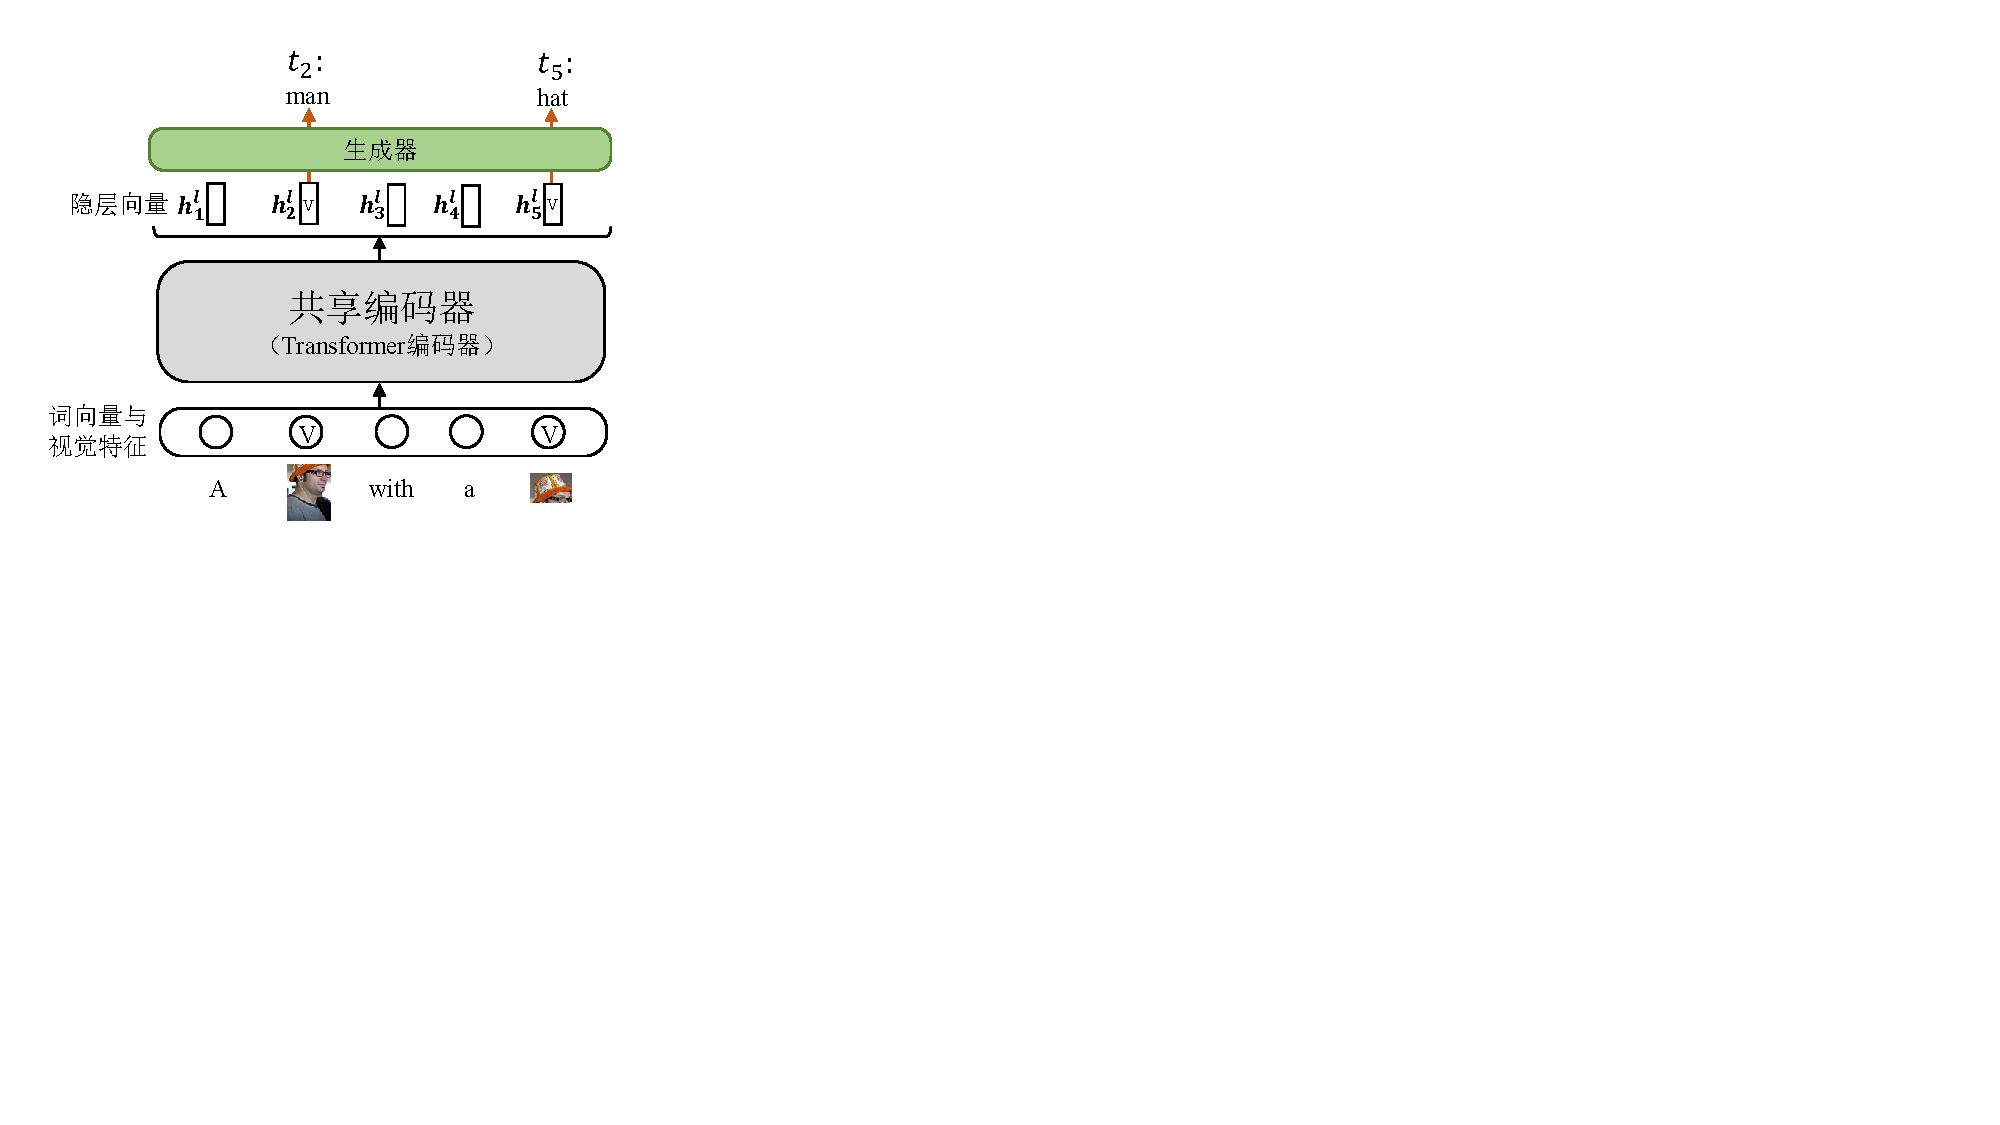
\includegraphics[scale=0.6]{Img/fig_4_ter.pdf}
    \bicaption{文本实体重构}{Textual entity reconstruction}
    \label{fig:4_ter}
\end{figure}
文本实体重构(Textual entity reconstruction,TER)与上一章相似,将视觉目标明确地作用到文本实体上。本章仅针对有对应视觉目标的名词采取实体替换,因此文本实体重构的输入为由文本上下文$\tilde{X}$和视觉实体$E$组合成的多模态混合序列:
\begin{equation}
Z={\rm{Combine}} \left( \tilde{X}, E \right)
\end{equation}
如图\ref{fig:4_ter}所示,输入的文本上下文“A <M> with a <M>”与视觉实体$\{e_1,e_5\}$组合成多模态混合序列$Z=$“A $e_1$ with a $e_5$”,此时输入到模型中的是三个空心圆代表词向量和两个标记“V”的圆代表视觉特征。多模态混合序列经过编码器进行跨模态编码后,得到序列的跨模态表示:
\begin{equation}
H_Z^L={\rm{MultiHead_{enc}^L}} \left( Z, Z, Z \right)
\end{equation}
其中,$H_Z^L=\{{\boldsymbol{h}_1^l},{\boldsymbol{h}_2^l},\cdots,{\boldsymbol{h}_N^l}\}$;${\rm{MultiHead_{enc}^L}} \left( \cdot,\cdot,\cdot \right)$代表$L$层采用多头注意力机制的编码器;$\boldsymbol{h}_i^l$中的$l$与$L$相同,代表第$l$层的编码结果。然后依据对应位置的隐层表示生成文本实体,在图2中为两个标记“V”矩形隐层表示${\boldsymbol{h}_2^l}$和${\boldsymbol{h}_5^l}$,该过程需要优化以下损失函数:
\begin{equation}
\mathcal{L}_{\rm{TER}} (\theta, \vartheta) =
    \frac{1}{{\vert}T{\vert}}
    \mathop{\sum}_{x_i \in T}
    {\rm{OH}} \left( x_i \right)
    {\rm log}{\ }{\rm p} \left( Z {\vert} \theta, \vartheta \right)
\end{equation}
\begin{equation}
{\log}{\ }{\rm p} \left( Z {\vert} \theta, \vartheta \right) =
    {\rm{g}} \left( {\boldsymbol h_i^l} \vert \vartheta \right)
\end{equation}
其中${\rm{OH}}\left(x_i\right)$代表$x_i$的独热编码(One-hot,OH)表示,$\theta$代表编码器一端的参数,$\vartheta$为生成器(Generator)参数,生成器${\rm{g}}\left(\cdot\right)$将位置$i$处的隐层向量${\boldsymbol{h}_i^l}$映射并得到词表中每个词的预测概率。

{\sffamily 视觉实体重构}

\begin{figure}[!htbp]
    \centering
    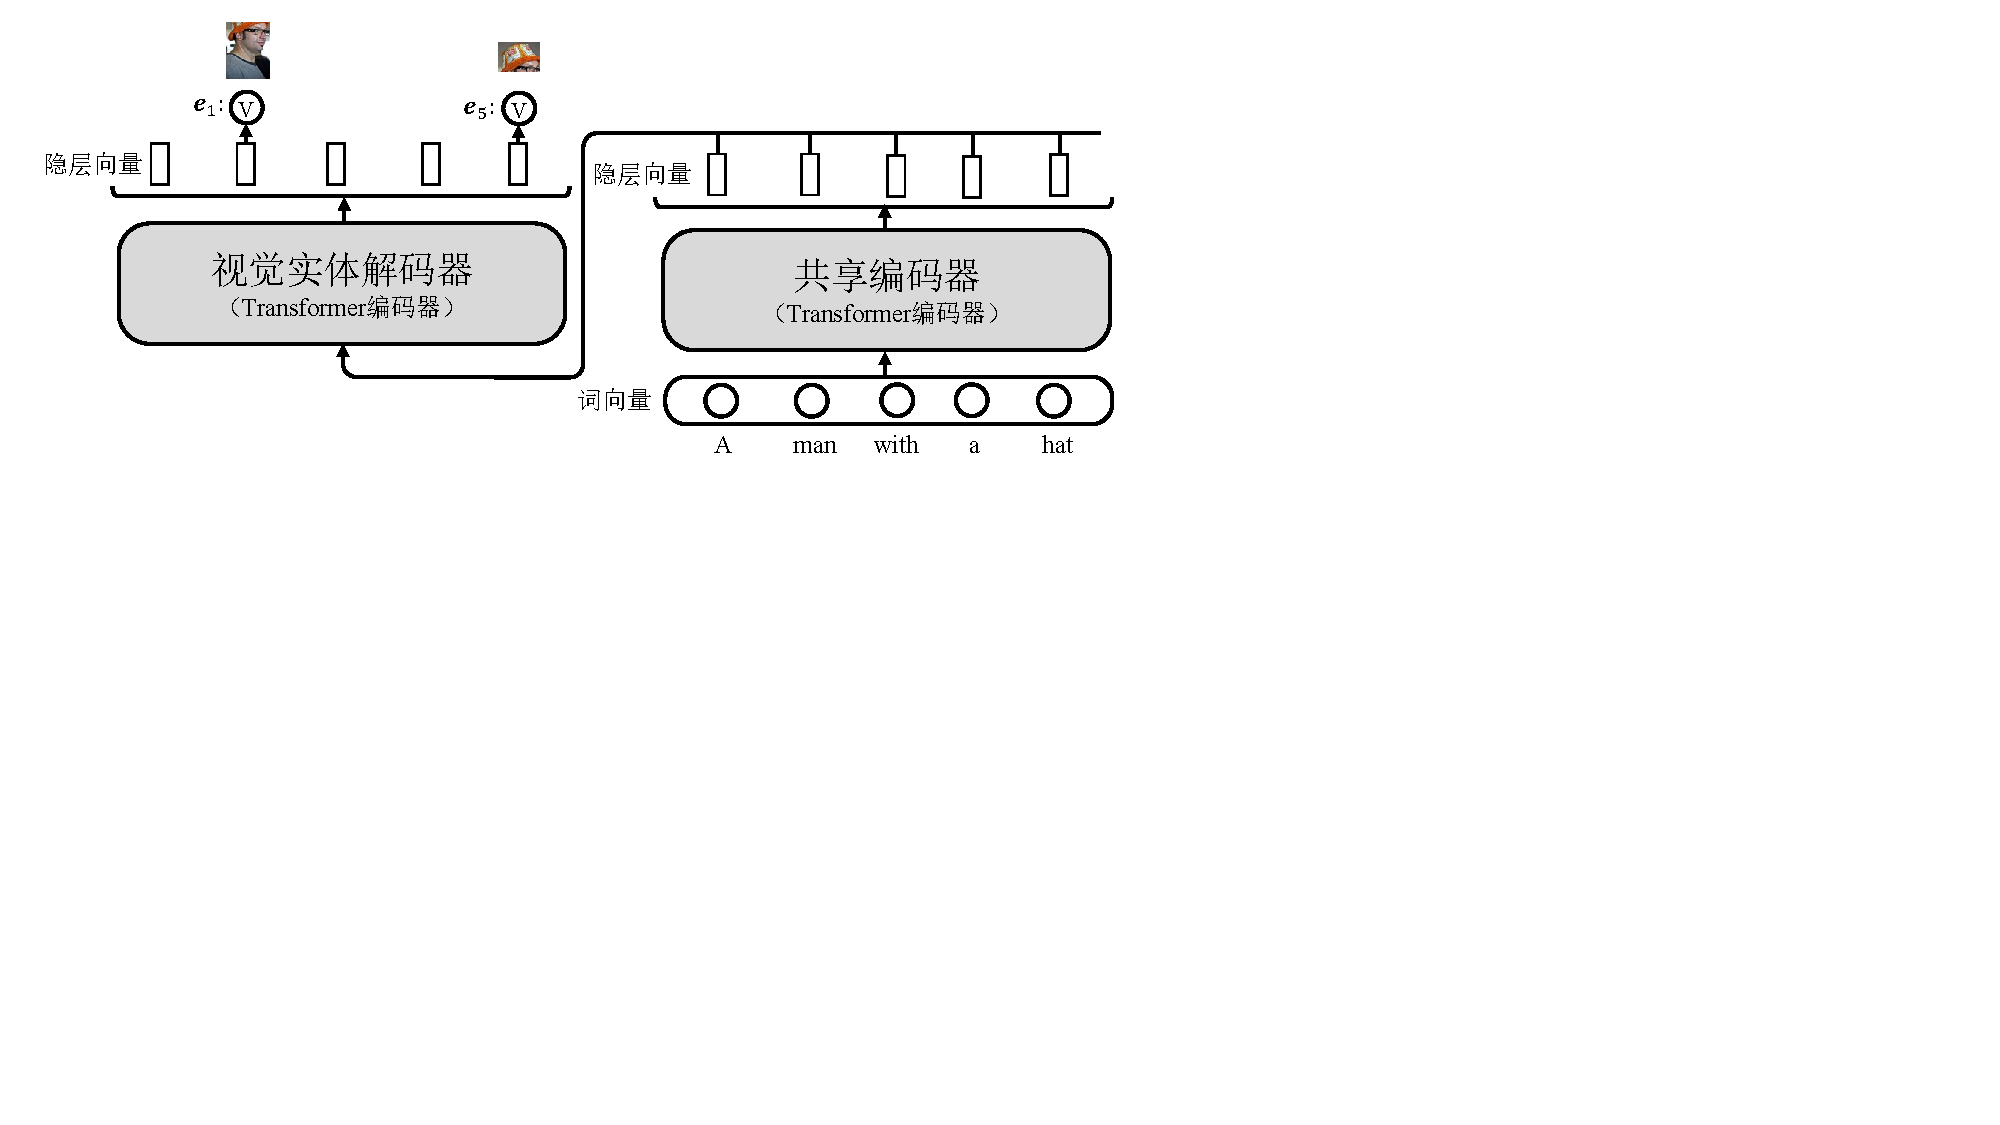
\includegraphics[scale=0.6]{Img/fig_4_ver.pdf}
    \bicaption{视觉实体重构}{Visual entity reconstruction}
    \label{fig:4_ver}
\end{figure}
与文本实体重构不同的是,视觉实体重构(Visual entity reconstruction,VER)依赖于来自单一的文本模态信息$X$。例如图\ref{fig:4_ver}中,“A man with a hat”为重构视觉实体时模型的输入序列,此时图中输入到模型中的是5个空心圆代表的词向量。该句子经过$L$层的编码器进行文本编码,再利用$L$层视觉实体解码器解码出与文本实体$\{t_1,t_5\}$相对应的视觉实体$\{e_1,e_5\}$。由于文本无法完整的描述图片,只是针对图片中的个别属性的描述,由文本直接还原像素级的图片或图片中的视觉实体几乎是不可能的。因此本文仅尝试生成与视觉实体相近的向量表示$\{{\boldsymbol{e}_1},{\boldsymbol{e}_5}\}$。其中,$X$经过如下编码过程:
\begin{equation}
H_X^L={\rm{MultiHead_{enc}^L}}(X, X, X)
\end{equation}
得到编码后的隐层表示$H_X^L=\{{\boldsymbol{h}_1^l},{\boldsymbol{h}_2^l},\cdots,{\boldsymbol{h}_N^l}\}$。然后经过如下解码过程:
\begin{equation}
H_X^{2L}={\rm{MultiHead_{dec}^L}}(H_X^L, H_X^L, H_X^L)
\end{equation}
得到$H_X^{2L}=\{{\boldsymbol{h}_1^{2l}},{\boldsymbol{h}_2^{2l}},\cdots,{\boldsymbol{h}_N^{2l}}\}$,${\rm MultiHead_{dec}^L}\left( \cdot,\cdot,\cdot \right)$为与${\rm MultiHead_{enc}^L}\left( \cdot,\cdot,\cdot \right)$具有相同结构的视觉实体解码器。然后利用$H_X^{2L}$生成与$\{{\boldsymbol{e}_a},{\boldsymbol{e}_b},\cdots\}$接近的向量表示,文本采用与文献\cite{37_elliott-kadar-2017-imagination}相近的方式实现该过程:
\begin{equation}
\mathcal{L}_{\rm{VER}}(\theta, \varphi)=
    \frac{1}{{\vert}E{\vert}}
    \mathop{\sum}_{j{\neq}i} {\max}\{0, \varepsilon - {\rm{cos}}\left( {\boldsymbol h_i^{2l}}, {\boldsymbol e_j} \right) + {\rm{cos}}\left( {\boldsymbol h_i^{2l}}, {\boldsymbol e_i} \right)\}
\end{equation}
%\onecolumn
%\input{docs/model_pic.tex}
%\begin{multicols}{2}
其中$i,j{\in}\{a,b,\cdots\}$为实体在句子中对应的序号;$\varphi$为视觉实体解码器的参数;${\rm{cos}}(\cdot,\cdot)$计算向量间的余弦相似度,$\varepsilon$为最小边缘常量。显然,优化$L_{\rm{VER}}(\theta,\varphi)$能够缩减${\boldsymbol{h}_i^{2l}}$与相对应的视觉实体${\boldsymbol{e}_i}$之间的余弦距离,增加与其它非对应的视觉实体${\boldsymbol{e}_j}$之间的余弦距离。

{\sffamily 文本非实体重构}

\begin{figure}[!htbp]
    \centering
    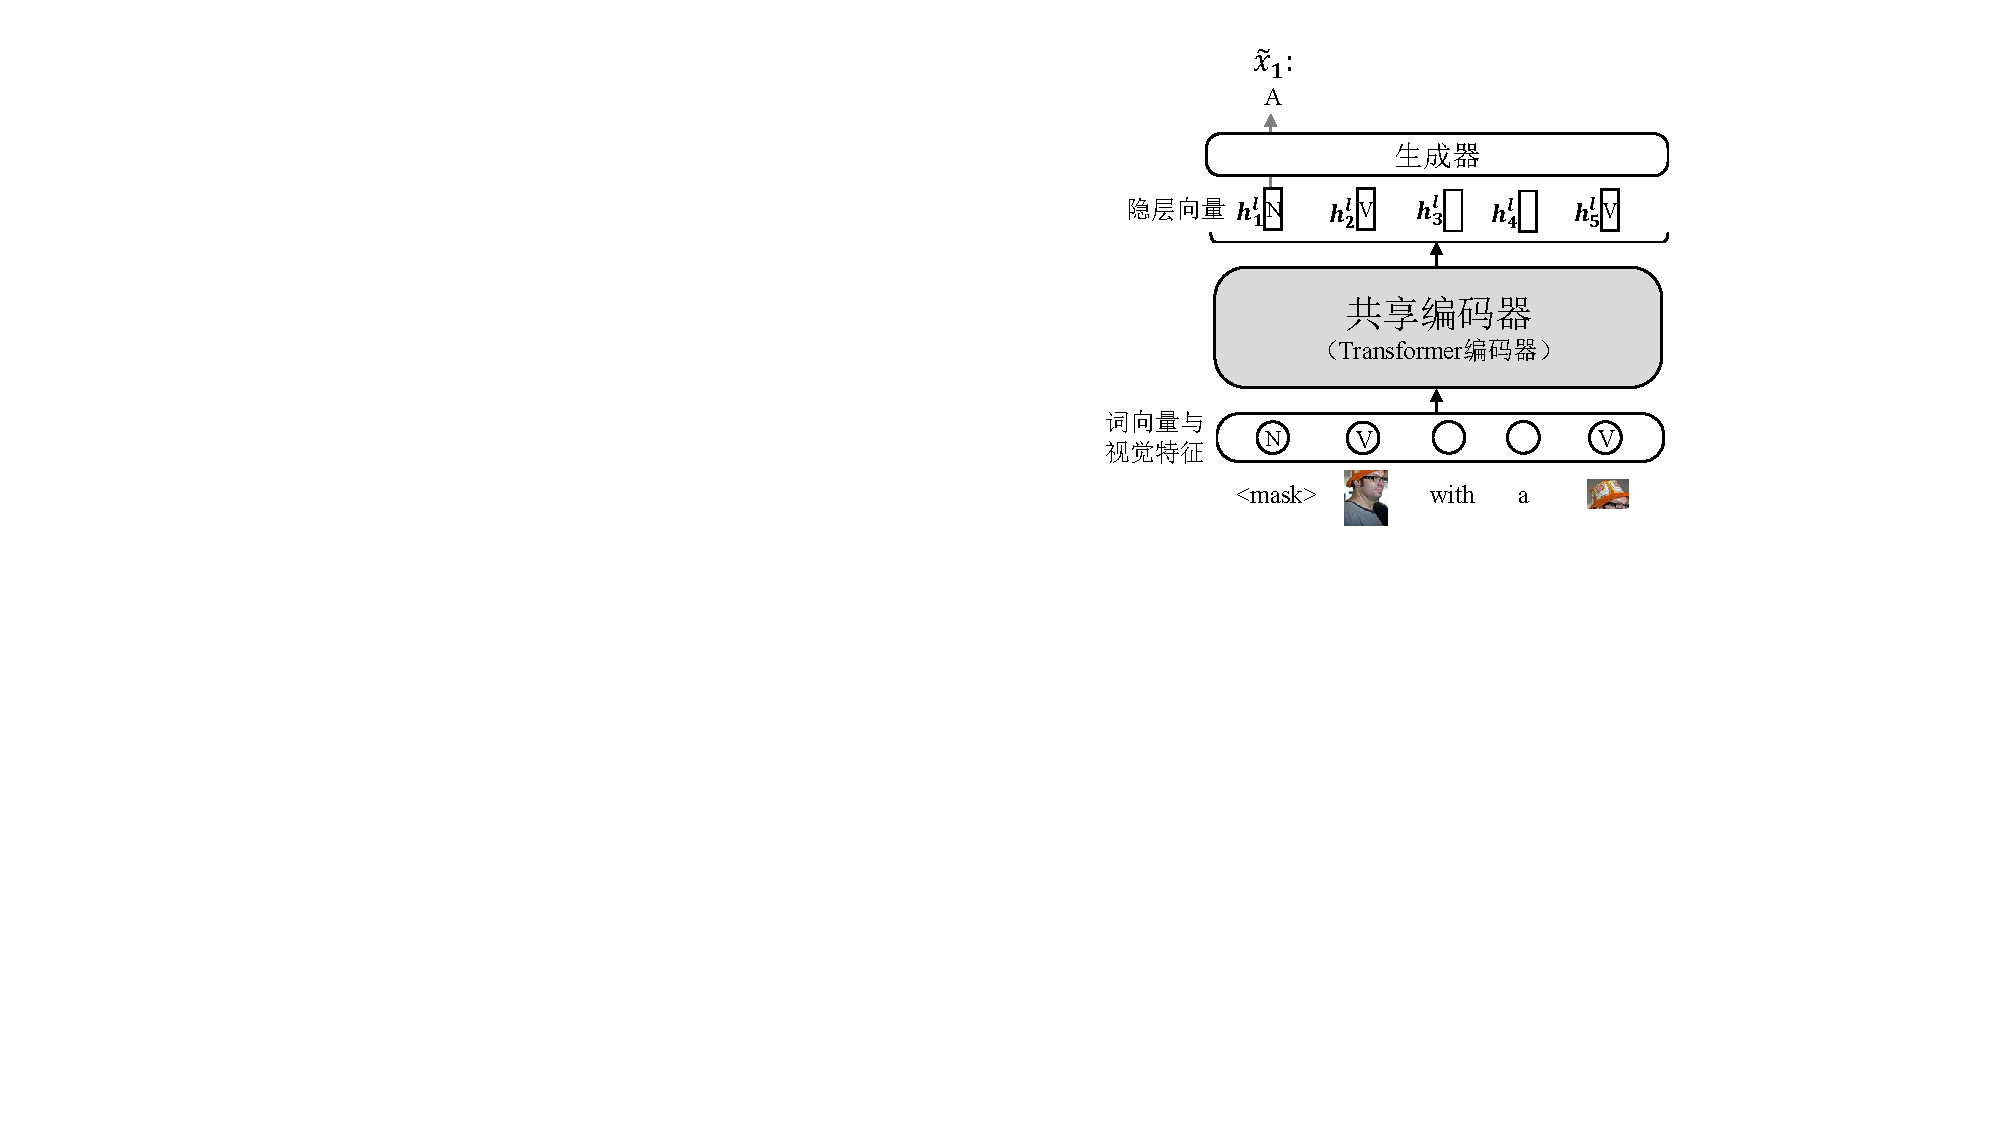
\includegraphics[scale=0.6]{Img/fig_4_tner.pdf}
    \bicaption{文本非实体重构}{Textual none-entity reconstruction}
    \label{fig:4_tner}
\end{figure}
文本非实体重构(Textual none-entity reconstruction,TNER)方法与文本实体重构方法相似,区别在于非实体重构的目的是使视觉实体与文本上下文进行充分的句子级语义融合,而实体的重构方法更侧重实体在两个模态之间的实体级语义融合。文本非实体的输入同样是文本上下文$\tilde{X}$和视觉实体$E$组合成的多模态混合序列,但是在$\tilde{X}$中除对实体的位置进行退化还要将待重构的非实体词退化。例如图2中,当选中对非实体词“A”进行重构时,模型所输入的多模态混合序列为$Z=$“<mask> $e_1$ with a $e_5$”,此时输入到模型中的是一个标记“N”的圆形,代表“<mask>”的词向量,以及两个空心圆形所代表的词向量和两个标记“V”的圆形所代表的视觉特征。损失函数如下:
%一个标记``N''的圆形词向量代表``$\langle$M$\rangle$''、两个圆形空心词向量和两个标记``V''的圆形视觉特征. 损失函数如下:
\begin{equation}
\mathcal{L}_{\rm{TNER}}(\theta, \vartheta) =
    \frac{1}{{\vert}\tilde{T}{\vert}}
    \mathop{\sum}_{x_i \in \tilde{T}}
    {\rm{OH}} \left( x_i \right)
    {\rm log}{\ }{\rm p} \left( \tilde{Z} {\vert} \theta, \vartheta \right)
\end{equation}
其中$\tilde{T}$代表待重构的非实体词集,并有$\tilde{T}\subseteq \tilde{X}$。在图2中用于预测非实体词“A”的隐层为一个标记“N”的矩形隐层表示${\boldsymbol{h}_1^l}$。

本文采用随机选取的方式选择待重构的非实体词。在执行TNER任务时,每个文本中的非实体词有$30\%$的概率会被选择到。该概率与所采用数据集中实体词占$32.6\%$的比例相近。

{\sffamily CER联合训练}

联合以上所有重构方法的目标函数,可得到本文所提CER方法的联合损失函数为:
\begin{equation}
\mathcal{L}_{\rm{CER}} \left( \theta, \varphi, \vartheta \right) = \alpha \mathcal{L}_{\rm{VER}} \left( \theta, \varphi \right) + \beta \mathcal{L}_{\rm{TER}} \left( \theta, \vartheta \right) + \gamma \mathcal{L}_{\rm{TNER}} \left( \theta, \vartheta \right)
\label{eq:4_combined_cer}
\end{equation}
其中,$\alpha$、$\beta$和$\gamma$为控制三种重构方法训练比例的超参数。值得注意的是,本文没有设置利用纯文本上下文$\tilde{X}$重构文本词的方案。这是因为该方案与一般的预训练方法相似,用于建立纯文本的语言模型。而机器翻译模型的编码端本身就是一个很好的纯文本语言模型,因此不必再设置纯文本的重构方案。

\subsection{与机器翻译相结合}
构建CER模型的目的是辅助翻译模型提升翻译质量。本文采用多任务训练方法将CER方法中的跨模态编码器与神经翻译模型的文本编码器进行参数共享,从而实现对神经机器翻译模型参数优化的目的。翻译任务所要优化的目标函数为:
\begin{equation}
\mathcal{L}_{\rm{NMT}} \left( \theta, \phi \right) =
    -\mathop{\sum}_j^M {\rm log}{\ }{\rm P} \left(y_j \vert y_{<j}, X \vert \theta, \phi \right)
\label{eq:4_nmt}
\end{equation}
其中$Y=\{y_1,y_2,\cdots,y_M\}$为目标语言的文本序列;$\phi$为解码器一端的参数,值得注意的是,在文本实体重构与文本非实体重构中所应用的生成器参数$\vartheta$是$\phi$的一部分,即采用的是同一个生成器。将公式\ref{eq:4_nmt}与CER模型的损失函数公式\ref{eq:4_combined_cer}相结合得到联合目标函数为:
\begin{equation}
\mathcal{L} \left( \theta, \phi, \varphi, \right) = \omega\mathcal{L}_{\rm{NMT}} \left( \theta, \phi \right) + \left( 1-\omega \right) \mathcal{L}_{\rm{CER}} \left( \theta, \varphi, \vartheta \right)
\end{equation}
其中,用超参数$\omega$调节神经机器翻译与CER方法的训练比例。
\section{实验设置}
\label{sec:4_setup}

\subsection{数据}
\label{sec:4_dataset}


\begin{table}[!htbp]
    \bicaption{Multi30K数据集情况统计}{Statistics about Multi30K dataset.}
    \label{tab:4_datasets}
    \centering
    \footnotesize% fontsize
    \setlength{\tabcolsep}{4pt}% column separation
    \renewcommand{\arraystretch}{1.2}%row space 
    \begin{tabular}{cccccc}
    \hline
      & \multirow{2}*{训练集} & \multirow{2}*{验证集} & \multicolumn{3}{c}{测试集} \\\cline{4-6}
      & & & Test2016 & Test2017 & MSCOCO \\\hline
    图片 & 29000 & 1014 & 1000 & 1000 & 461 \\
    英语 & $\checkmark$ & $\checkmark$ & $\checkmark$ & $\checkmark$ & $\checkmark$ \\
    德语 & $\checkmark$ & $\checkmark$ & $\checkmark$ & $\checkmark$ & $\checkmark$ \\
    法语 & $\checkmark$ & $\checkmark$ & $\checkmark$ & $\checkmark$ & $\checkmark$ \\
    捷克语 & $\checkmark$ & $\checkmark$ & $\checkmark$ &   &   \\
     \hline
    \end{tabular}%
\end{table}%

本章使用多模态机器翻译任务的常用数据集Multi30K\cite{43_elliott-etal-2016-multi30k}来测试本文所提方法。该数据集每张图片配有一个英文句子和其对应的德语、法语和捷克语的译文。该数据集的训练集包含29000个平行句对。其验证集和测试集Test2016的大小分别为1014和1000。常用的测试集还包括Multi30K Test2017以及Ambiguous MSCOCO上进行了测试,其大小分别为1000和461。数据集的具体统计情况如表\ref{tab:4_datasets}所示。值得注意的是,在融合图片信息的神经机器翻译任务中,最常用的是英德翻译数据。其次是英法翻译数据,相应的翻译准确率的比较多数是在Test2016测试集上进行的。而英捷翻译数据仅有很少的应用。

本文采用Moses SMT\cite{44_koehn-etal-2007-moses}工具包对文本数据进行分词和归一化处理。为了防止对视觉实体与文本实体对应关系的破坏,本文并没有采用双字节编码\cite{27_sennrich-etal-2016-neural}(Byte pair encoding,BPE)进行分词处理。在数据的预处理阶段,本文采用上一章\ref{sec:3_entity_extraction}节所介绍的方法提取文本实体与视觉实体,并将它们对应起来。最后将视觉实体输入Resnet-50\cite{32_DBLP:conf/cvpr/HeZRS16}提取出2048维的全局图像特征,该特征向量在输入到CER模型的时候会通过一个全连接层映射到模型所需的维度。

\subsection{模型参数}
\label{sec:4_model_setup}

本文在基于Transformer\cite{5_DBLP:journals/corr/VaswaniSPUJGKP17}结构的模型上进行试验。由于数据集Multi30K的规模相对较小,很容易在Transformer-big或Transformer-base上过拟合,因此本章采用了更小规模的参数设置。本文所设置的参数与文献\cite{33_yin-etal-2020-novel}基本保持一致,其词嵌入层设置为128维,前馈内层为256维。编码器、视觉实体解码器和翻译解码器均为4层,多头自注意力的头数为4。词表采用源语言与目标语言共享的方式,合并后英译德的共享词表大小为27226,英译法为19393,英译捷为29170。利用Adam\cite{34_DBLP:journals/corr/KingmaB14}优化器优化整个模型参数。本章与文献\cite{5_DBLP:journals/corr/VaswaniSPUJGKP17}相同采用预热和衰减策略来提高学习率,预热步骤为4000,总训练步骤为80000。训练目标中设置平滑标签$\epsilon_{ls}=0.1$。训练时,批数据大小为2000个单词。测试时,采用了搜索空间$b=4$的柱搜索算法。

多任务学习方法的训练方式为随机选择一个任务在当前批数据下对模型进行优化。本文所提CER方法一共包含三个子任务:VER、TER和TNER。这三个任务根据超参数$\alpha$、$\beta$和$\gamma$控制训练的比例。本文将三个子任务的训练比例设置为$\alpha=40\%$、$\beta=40\%$和$\gamma=20\%$。这样保证了CER在训练中将实体键的跨模态信息融合作为主任务,以$80\%$的比例用于跨模态实体重构,$20\%$的比例用于视觉实体与非实体上下文的语义融合。本文将翻译任务设置为主任务,并设置超参数$\omega$为控制翻译任务与CER之间的训练比重。例如当$\omega=0.5$时,NMT与CER的训练比例分别为$50\%$,其中VER、TER和TNER三个子任务的训练比重依据上文调整为$\omega\times\alpha=20\%$、$\omega\times\beta=20\%$和$\omega\times\gamma=10\%$。

%本文所有的模型结果都是在3次随机初始化的条件下训练得到的平均值。最后,通过BLEU4$^{[32]}$和METEOR$^{[33]}$来测试翻译质量,在后面的实验中分别简化为``B''和``M''。


\subsection{对比模型}
\label{sec:4_comparison}

本章将对比方法分为图片信息辅助式和图片信息增强式两类方法。图片信息辅助式方法在训练和测试时均使用额外的图片输入作为上下文信息提升模型的翻译准确率。图片信息增强式则只需要在训练阶段输入图片,通过优化翻译模型的参数来提升模型最终的纯文本翻译质量。本章所提方法属于图片信息增强式方法。图片信息辅助式方法的介绍如下:
%本文将MMT方法分为句子级融合、视觉实体融合以及增强NMT三大类。句子级融合方法主要尝试将视觉信息与整个文本句子进行语义融合。视觉实体融合方法则提预先提取出图片中的视觉目标后再输入到所设计的模型中。增强NMT方法一般在训练中融合视觉信息,而在测试时不需要输入图片。后两类方法中的多数模型在本质上也属于句子级融合方法。各模型简介如下:

\begin{itemize}

\item \textbf{SerialAtt\cite{47_DBLP:conf/wmt/LibovickyHM18}:}该模型在解码过程中采用了多个交叉注意力串联的形式,每个交叉注意力模块对应了不同的信息来源。在融合图片信息的模型中,两个交叉注意力模块分别用于采集源语言和图片中的信息。

\item \textbf{DelMMT\cite{39_ive-etal-2019-distilling}}模型提出使用推敲网络做多模态二次解码。在第二次解码中融合源语言、目标语言以及视觉信息。

\item \textbf{GAMMT\cite{41_DBLP:journals/corr/abs-2103-08862}:}使用Gumbel-Sigmoid改造注意力机制,帮助翻译模型关注到图片中与文本内容更相关的区域。

\item \textbf{GMMT\cite{33_yin-etal-2020-novel}:}该模型视源语言句子与图片中的视觉目标为一个多模态图结构,然后利用设计的基于图的跨模态编码器进行编码,最终解码出目标端句子。
\end{itemize}

图片信息增强式方法的介绍如下:
\begin{itemize}
\item \textbf{Transformer:}基于Transformer的纯文本神经机器翻译模型,其模型配置与\ref{sec:4_model_setup}小节保持一致。
\item \textbf{Imagination\cite{37_elliott-kadar-2017-imagination}:}该方法将源语言句子编码后,利用编码后的隐层表示生成与图片的全局特征相近的向量表示,该过程称为“想象力”机制。该方法同样使用了多任务的方式。
\item \textbf{ImagiT\cite{51_long-etal-2021-generative}:}该方法同样采用了“想象力”机制,区别在于ImagiT采用了生成对抗网络,尝试从对原文的编码中“想象”出像素级的图片。
\item \textbf{CTR-NMT:}该模型为本文第3章所设计的方法,采用了词级实体替换方案利用独享解码器重构源语言,是一种图片增强式神经翻译模型。
\end{itemize}
\section{实验结果}

\subsection{超参数$\omega$的影响}
\label{sec:4_omega}
本章提出的多任务训练方法包含了翻译和CER两个由超参数$\omega$控制训练比例的任务,而CER又包含了TER、VER和TNER三个由$\alpha$、$\beta$和$\gamma$三个超参数控制的子任务。因此如何平衡这些任务的训练比重是在模型训练过程中极为重要的问题。本章根据三个子任务的重要程度,将$\alpha$、$\beta$和$\gamma$三个超参数的比例固定为$2:2:1$,然后通过调节超参数$\omega$来寻找翻译和CER两个任务合适的训练比例。本节依据CER-NMT在英德翻译验证集上的BLEU值结果来选取一个合适的$\omega$值。

%\begin{figure}[!htbp]
%    \centering
%    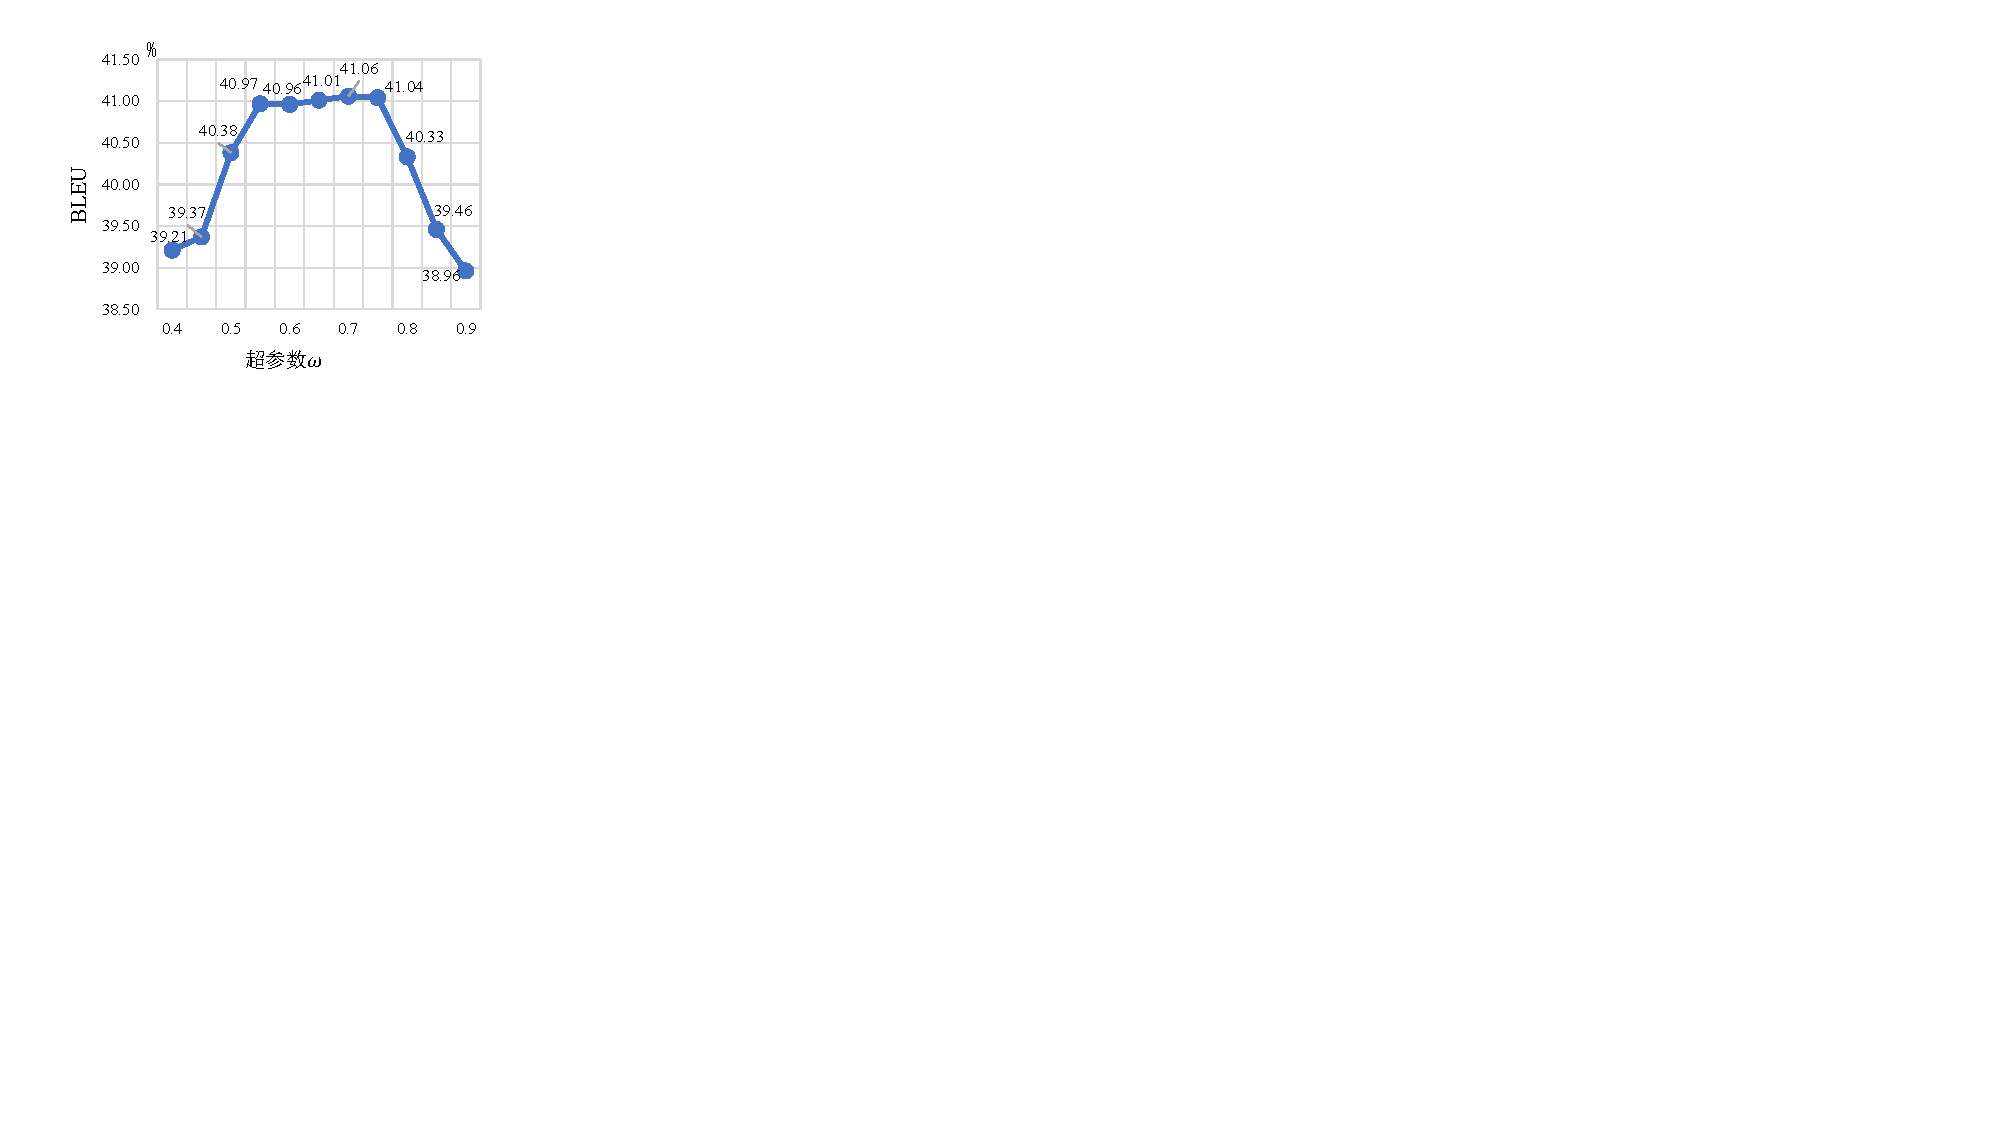
\includegraphics[scale=1.2]{Img/fig_4_searchw.pdf}
%    \bicaption{超参数$\omega$对CER-NMT翻译准确率的影响}{Effect of hyperparameter $\omega$ on translation accuracy of CER-NMT}
%    \label{fig:4_searchw}
%\end{figure}


\begin{figure}[!htbp]
    \centering
    \begin{subfigure}[b]{0.5\textwidth}
      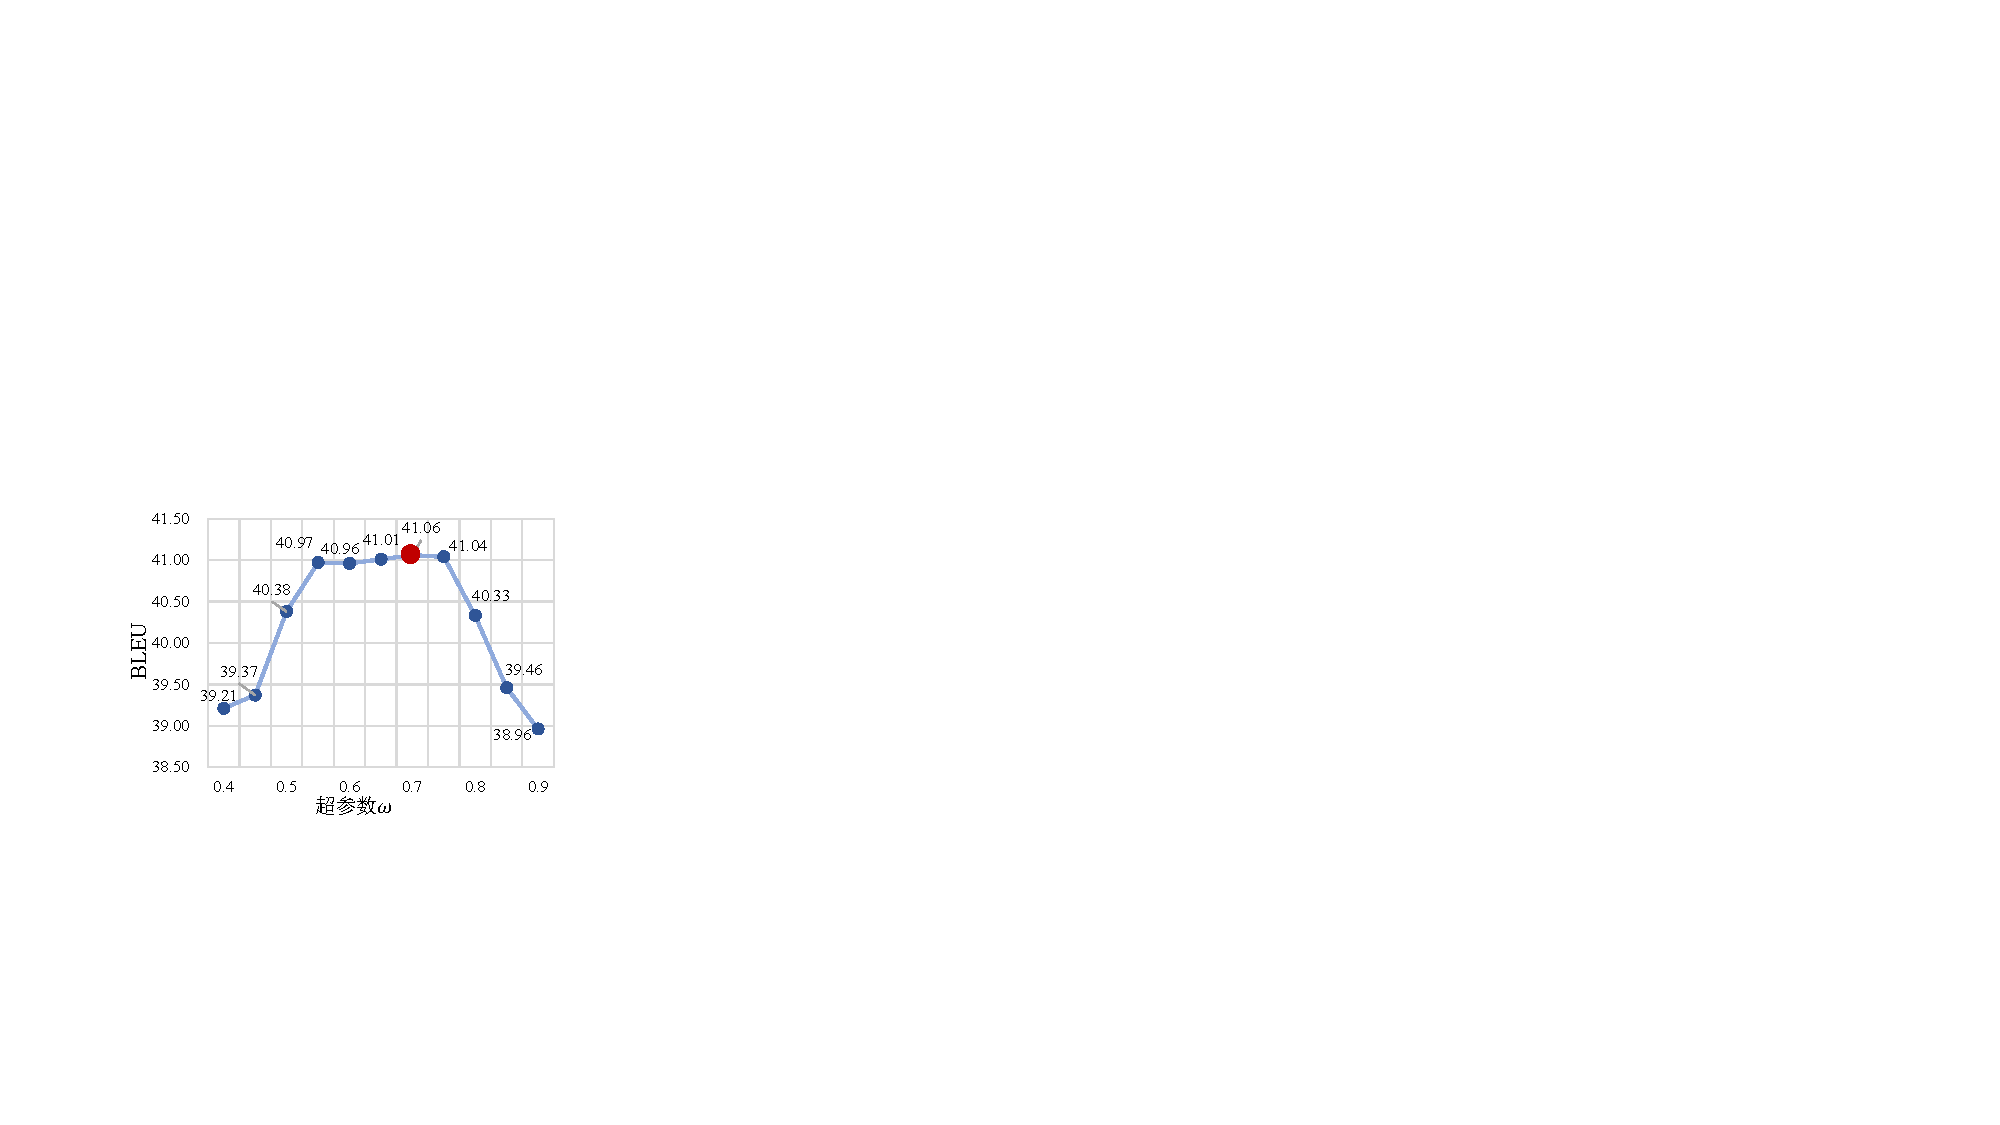
\includegraphics[width=\textwidth]{Img/fig_4_searchw_ende.pdf}
      \caption{英德翻译}
      \label{fig:4_searchw_ende}
    \end{subfigure}%
    ~% add desired spacing
    \begin{subfigure}[b]{0.5\textwidth}
      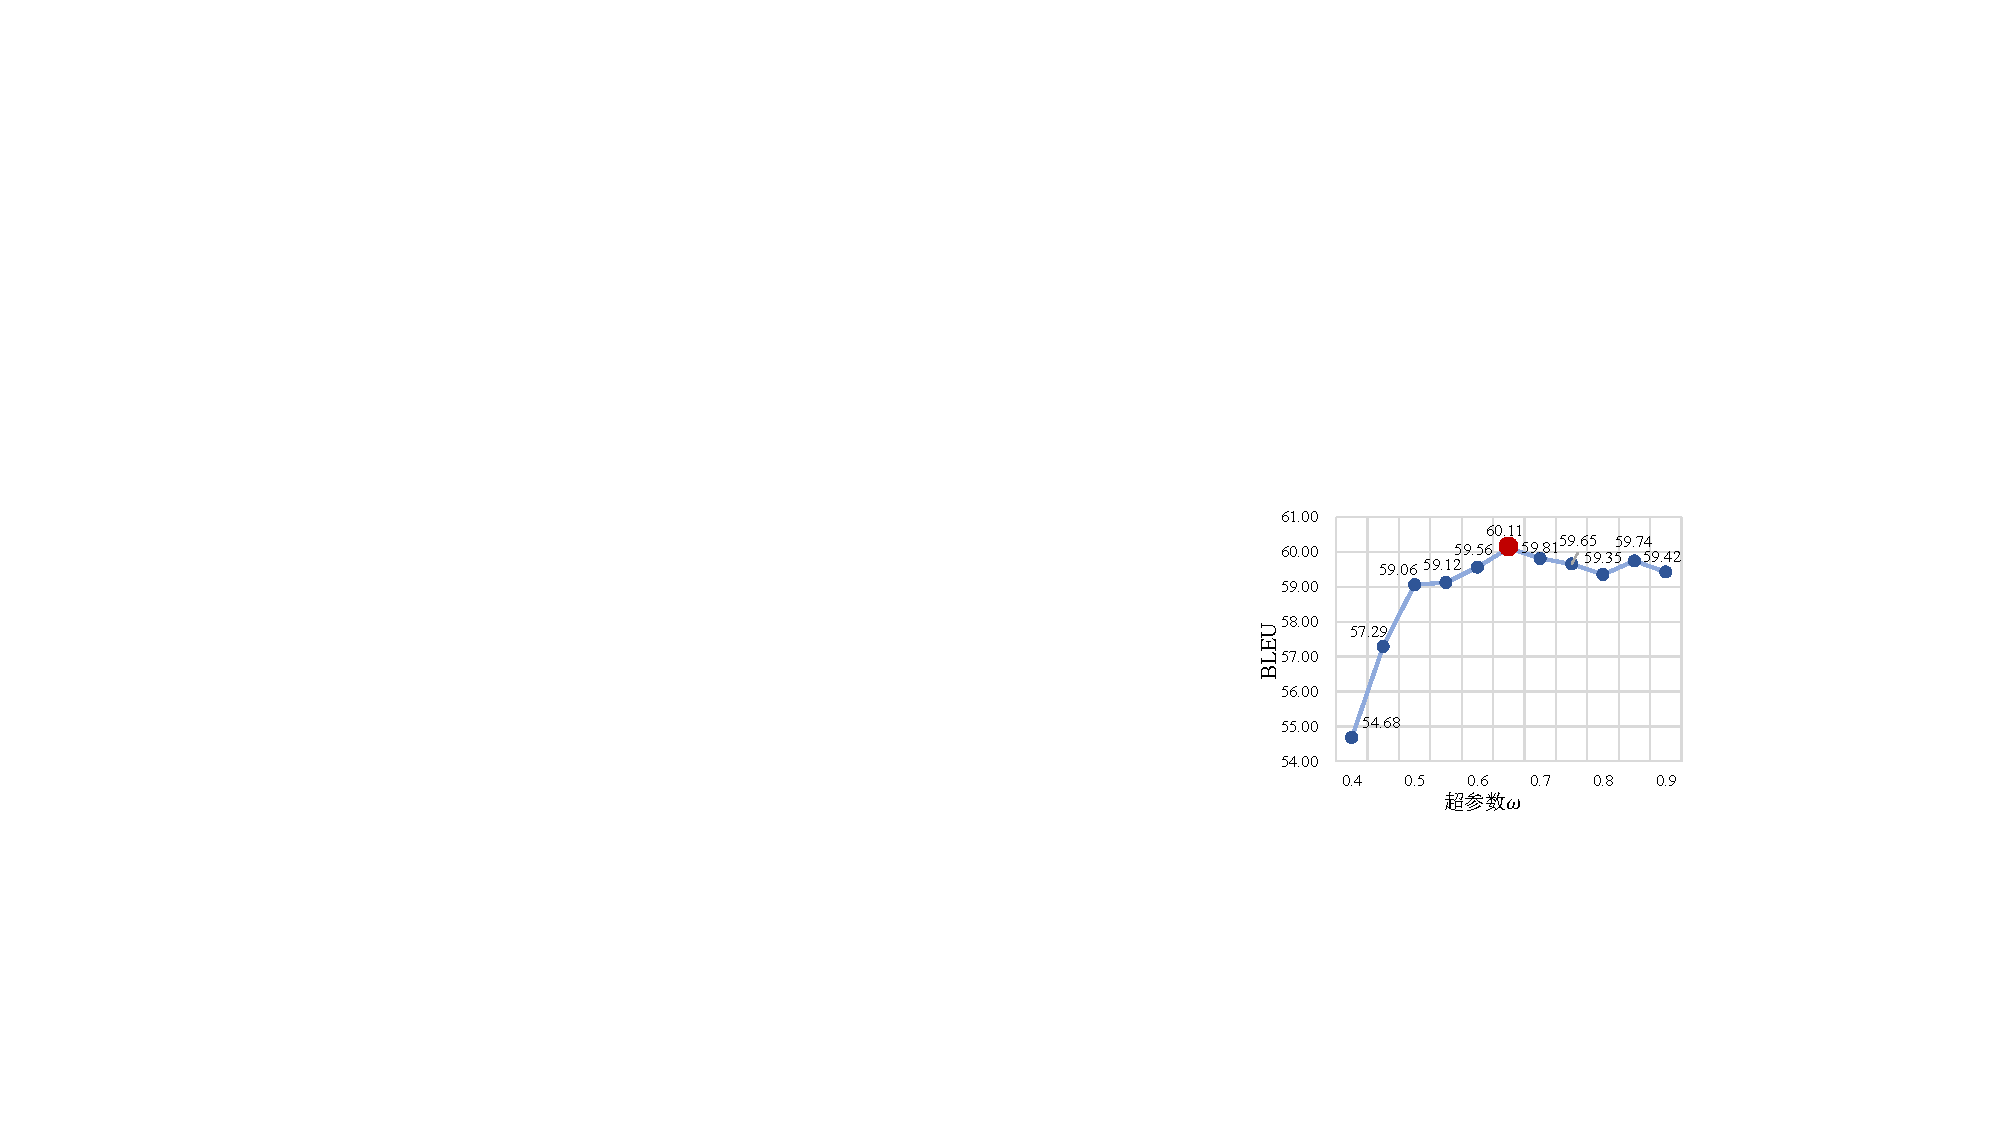
\includegraphics[width=\textwidth]{Img/fig_4_searchw_enfr.pdf}
      \caption{英法翻译}
      \label{fig:4_searchw_enfr}
    \end{subfigure}
    \\% line break
    \begin{subfigure}[b]{0.5\textwidth}
      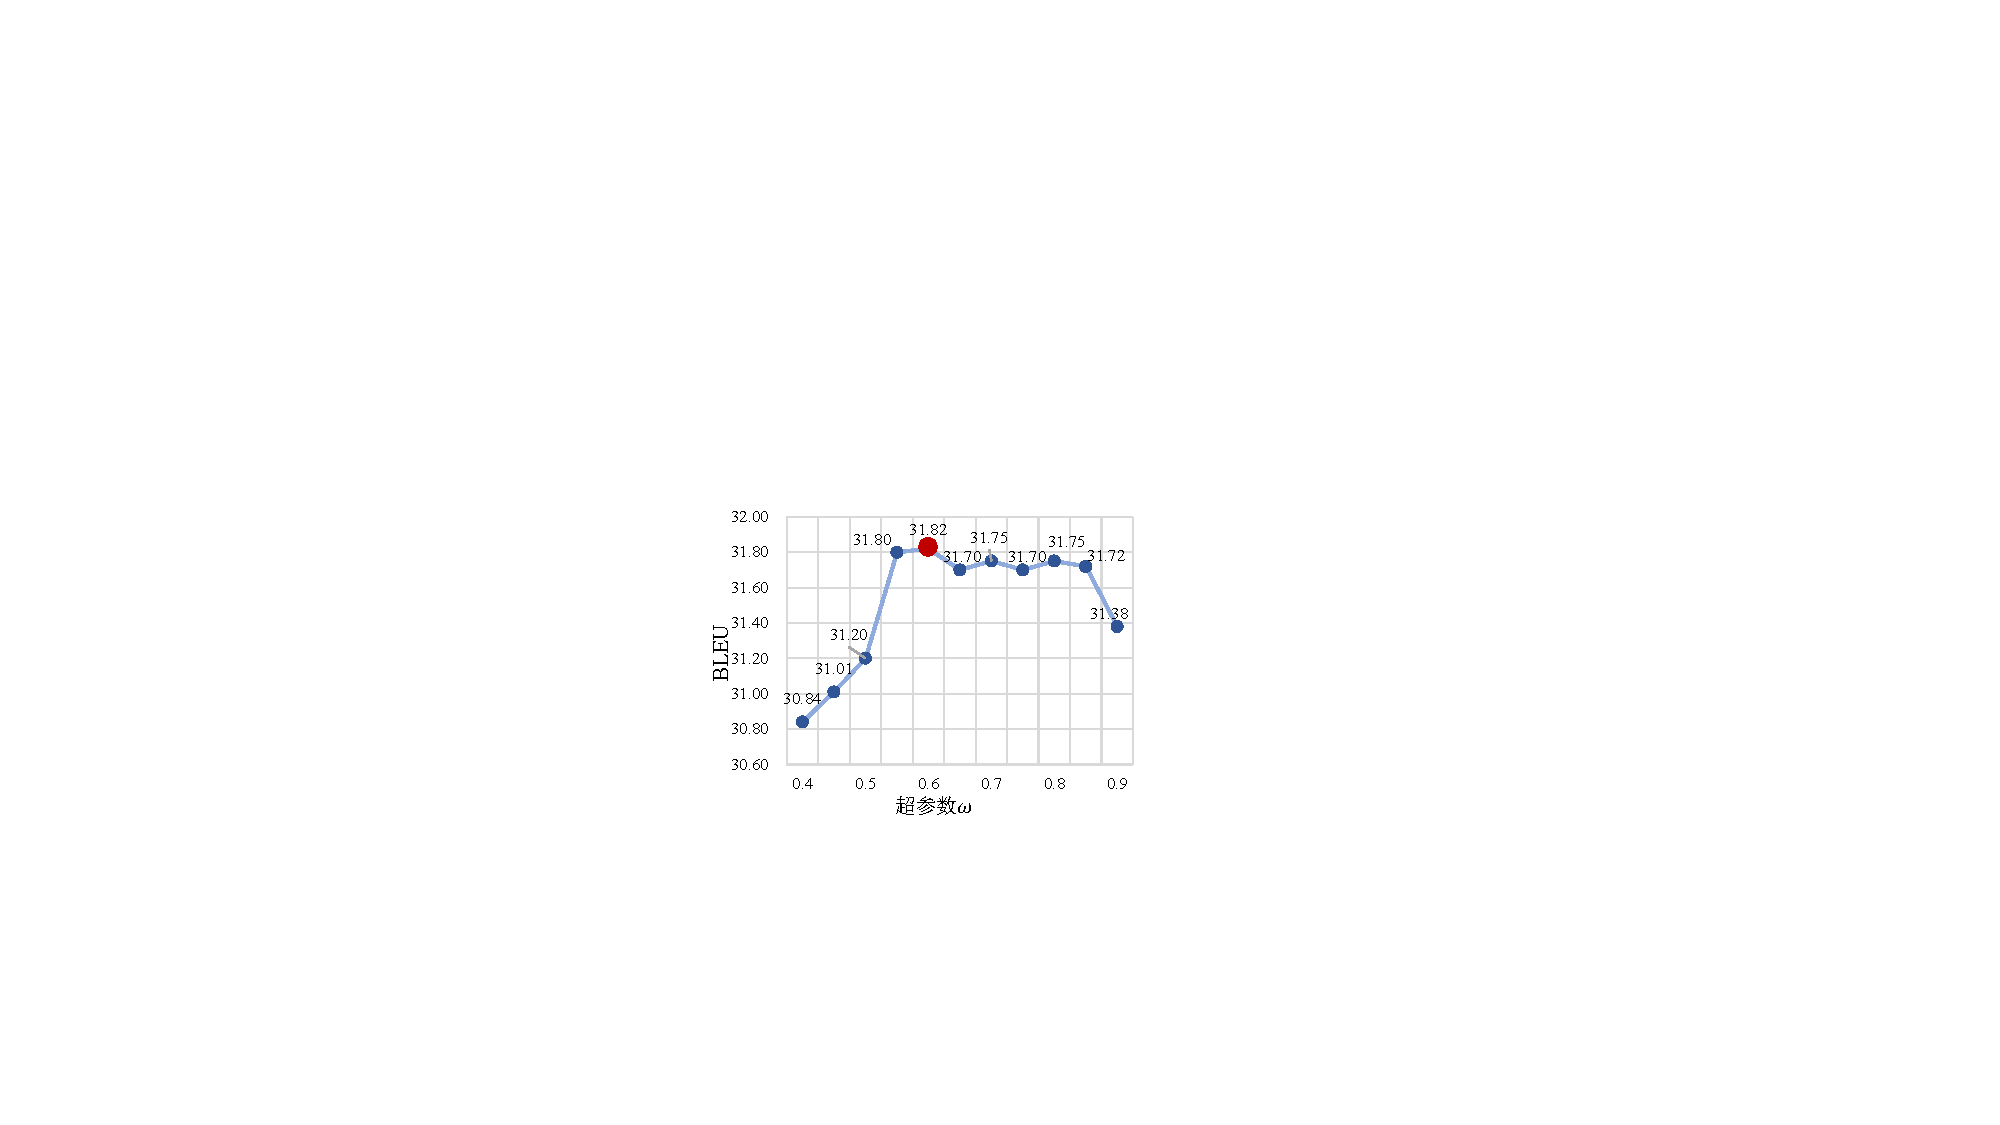
\includegraphics[width=\textwidth]{Img/fig_4_searchw_encs.pdf}
      \caption{英捷翻译}
      \label{fig:4_searchw_encs}
    \end{subfigure}%
    \bicaption{超参数$\omega$对CER-NMT翻译准确率的影响}{Effect of hyperparameter $\omega$ on translation accuracy of CER-NMT}
    \label{fig:4_searchw}
\end{figure}
如图\ref{fig:4_searchw}所示实验结果,横轴代表$\omega$从0.4以0.05为间隔增加至0.9,纵轴为NMT模型在英译德验证集上的BLEU值。当$\omega=1.0$时,代表翻译任务的训练比例为$100\%$,此时是纯文本神经机器翻译。当$\omega=0.0$时,代表仅训练CER不做翻译。该图反映出,当$\omega \in [0.5,0.8]$时,模型均具有较好的效果。超过这个范围时,CER-NMT的BLEU值将逐渐接近纯文本翻译模型。低于这个范围时,CER-NMT的翻译准确率发生了骤减。我们还测试了当$\omega=0.3$时的情况,此时BLEU值以骤减到9.86。以上实验结果说明在一个合适的范围内,CER方法能够帮助翻译模型提升翻译准确率。而这个范围应当使模型的训练过程主要以翻译任务为主以CER为辅。因此,本章选择$\omega=0.7$,即CER-NMT在验证集上达到最高的BLEU值时,作为后续试验中对超参数$\omega$的设置。


\subsection{翻译结果}
\label{sec:4_ende}


\begin{table}[!htbp]
    \bicaption{在Multi30K英德翻译上的结果。}{Translation results on Multi30K EN-DE.}
    \label{tab:4_ende_enfr}
    \centering
    \footnotesize% fontsize
    \setlength{\tabcolsep}{4pt}% column separation
    \renewcommand{\arraystretch}{1.2}%row space 
\begin{tabular}{ccccccccc}
\hline
 \multirow{3}{*}{模型} & \multicolumn{6}{c}{英译德} & \multicolumn{2}{c}{英译法} \\
\cmidrule(r){2-7} \cmidrule(r){8-9}%\hline
       & \multicolumn{2}{c}{Test2016} & \multicolumn{2}{c}{Test2017} & \multicolumn{2}{c}{MSCOCO} & \multicolumn{2}{c}{Test2016} \\
\cline{2-9}%\cmidrule(r){2-7} \cmidrule(r){8-9} %\cline{2-9}
              &    BLEU & METEOR &     BLEU & METEOR &     BLEU & METEOR &     BLEU & METEOR \\
\hline
\multicolumn{9}{c}{图片信息辅助式方法} \\
\hline
SerialAtt      & 38.7 & 57.2 & - & - & - & - & 60.8 & 75.1 \\
DelMMT           & 38.0 & 55.6 & - & - & - & - & 59.8 & 74.4 \\
GAMMT      & 39.2 & {\textbf{57.8}} & 31.4 & 51.2 & 26.9 & 46.0 & - & - \\
GMMT             & 39.8 & 57.6 & 32.2 & 51.9 & 28.7 & {\textbf{47.6}} & 60.9 & 74.9 \\
\hline
\multicolumn{9}{c}{图片信息增强式方法} \\
\hline
Imagination      & 36.8 & 55.8 & - & - & - & - & - & - \\
ImagiT   & 38.6 & 55.7 & 32.1 & {\textbf{52.4}} & - & - & 59.9 & 74.3 \\
CTR-NMT             & 39.7 & 57.5 & {\textbf{32.9}} & 51.7 & {\textbf{29.1}} & 47.5 & 61.1 & 75.8 \\
\hline
\multicolumn{9}{c}{本章所提方法} \\
\hline
Transformer             & 38.5 & 57.5 & 31.0 & 51.9 & 27.5 & 47.4 & 60.5 & 75.6 \\
CER-NMT          & {\textbf{40.2}} & {\textbf{57.8}} & 32.5 & 52.0 & 28.3 & 47.1 & {\textbf{61.6}} & {\textbf{76.1}} \\
\bottomrule
\end{tabular}
\end{table}

表\ref{tab:4_ende_enfr}显示了采用了CER方法的NMT系统的翻译结果。其中$\omega$按照4.1节的结论取值为0.7,对应的VER、TER和TNER三个子任务的训练比重分别为$12\%$、$12\%$和$6\%$。


表\ref{tab:4_ende_enfr}中加粗项表示整列中的最佳结果。根据以上英译德和英译法的实验结果可以得到以下结论:

%\begin{itemize}
%\item
(1)本章所提方法在Multi30K Test2016测试集的英德翻译和英法翻译两种语言对上取得了BLEU和METEOR的最佳结果,并且在Test2017测试集上的结果超过了多数模型的结果,并与其它模型的最佳结果相比差距很小。这说明CER方法能够有效提升NMT模型的翻译质量。

%\item
(2)CER-NMT在歧义词较多的Ambiguous MSCOCO上的表现并不理想,落后于GMMT和上一章的CTR-NMT两个模型。这是因为CER方法主要帮助翻译模型在训练阶段融合视觉信息,在测试阶段因为不需要输入图像使得模型无法借助视觉信息解决歧义词的问题。同理可以看到,CTR-NMT在METEOR上的提升也仅有0.1。这说明图片信息增强式的方法虽然能够提升模型的翻译质量,但也同样具有一定的局限性。例如文本中常见的歧义词问题或语义不完整问题,是需要利用图片信息辅助翻译模型来解决。

(3)%\item
GMMT、CTR-NMT和CER-NMT均是采用视觉目标作为视觉输入的方法,其结果均优于采用完整图片输入的方法。理想的情况下,完整的图片包含的视觉信息更完整,对翻译带来的好处会更多。但是目前实验结果说明,在神经机器翻译中融合图片信息是非常困难的,需要为NMT模型提供更细粒度的视觉信息才能降低跨模态信息融合的难度,使模型更多地利用图片中的视觉信息。
%\end{itemize}

综合以上的实验结果,本章所提的跨模态实体重构方法能有效地提升机器翻译的质量。同时也说明了虽然图片信息增强式的翻译方法无法解决歧义词和语义不完整问题,但是方法的有效性也体现了图片信息具有除补全语以外的其它作用。

\subsection{消融实验}
\label{sec:4_ablation_study}
为了探究VER、TER和TNER三个子任务对CER$-$NMT模型的影响,本节设置了12组消融实验。其中序号0代表4.2节中CER-NMT的结果。序号1$-$3组各去掉一个子任务,并保持剩余子任务的训练权重。序号4$-$5组各去掉一个子任务,保持NMT的权重。序号7$-$9组各保留一个子任务,保持子任务的权重。序号10$-$12组保留一个子任务,保持NMT的权重。

\begin{table}[!htbp]
    \bicaption{在Multi30K Test2016英德翻译上消融实验}{Ablation study on the EN-DE of Multi30K Test2016}
    \label{tab:4_ablation_study}
    \centering
    \footnotesize% fontsize
    \setlength{\tabcolsep}{8pt}% column separation
    \renewcommand{\arraystretch}{1.2}%row space 
\begin{tabular}{cccccc}
\hline
\multirow{2}{*}{序号} & NMT & VER & TER & TNER & \multirow{2}{*}{BLEU} \\
\cline{2-5}
   & $\omega$ & $\omega \times \alpha$ & $\omega \times \beta$ & $\omega \times \gamma$ & \\
\hline
0  & 0.70 & 0.12 & 0.12 & 0.06 & 40.2 \\
\hline
1  & 0.76 & 0.12 & 0.12 &  -   & 40.0 \\
2  & 0.82 & 0.12 & -    & 0.06 & 39.5 \\
3  & 0.82 & -    & 0.12 & 0.06 & 39.6 \\
\hline
4  & 0.70 & 0.15 & 0.15 & -    & 39.9 \\
5  & 0.70 & 0.20 & -    & 0.10 & 39.2 \\
6  & 0.70 & -    & 0.20 & 0.10 & 39.3 \\
\hline
7  & 0.88 & 0.12 & -    & -    & 38.8 \\
8  & 0.88 & -    & 0.12 & -    & 38.8 \\
9  & 0.94 & -    & -    & 0.06 & 39.0 \\
\hline
10 & 0.70 & 0.30 & -    & -    & 39.2 \\
11 & 0.70 & -    & 0.30 & -    & 39.4 \\
12 & 0.70 & -    & -    & 0.30 & 39.0 \\
\hline
\end{tabular}
\end{table}

实验结果如表2所示,其中“-”代表所对应的子任务被去掉,可以获得如下信息:

%\begin{itemize}
%\item
(1)序号1$-$6组各去掉了一个子任务,序号7$-$12组各仅保留一个子任务。从两组之间的对比可以看出,1$-$3的结果整体优于7$-$8,4$-$6的结果整体优于10$-$12,说明无论是保持子任务的训练比重不变还是保持翻译任务的训练比重不变,子任务组合的方式总是优于仅使用单一的子任务。其中,VER和TER的在序号1和4中的组合已经可以使翻译模型得到很好的结果。TNER对NMT的影响最小,但是依旧可以为NMT模型带来小幅度的提升。

%\item
(2)$\omega>0.8$的实验组2,3,7,8,9的结果与\ref{sec:4_omega}小节中的实验结果均说明减少跨模态任务至一定比重后,模型的翻译准确率将逐渐趋近于纯文本翻译模型。

%\item
(3)与\ref{sec:4_ende}小节中CER-NMT的实验结果相比可以说明,针对实体重构的VER和TER任务对翻译模型的性能影响最大,且这两个任务组合情况下的结果要优于单独使用的情况。相比之下,TNER同样可以为翻译性能带来一定的提升,但效果不如实体重构明显。综合以上,TER、VER和TNER三个子任务共同配合可以使翻译模型的性能达到最佳。
%\end{itemize}


\subsection{文本实体忠实度}
\label{sec:4_fidelity}
本章所提方法对视觉实体与文本实体互相结合跨模态信息,再将视觉实体与文本上下文相融合。而这一过程中是以实体间的信息融合为主导的,\ref{sec:4_ablation_study}小节的实验也证实了这一点。这使得视觉信息具有明确的作用方向。因此检验视觉信息是否对文本实体的翻译产生了影响成为了一个必要的环节。本节我们将尝试测量在解码生成目标单词时对文本实体的忠实度来反映模型的行为变化。

Transformer的解码器采用的是交叉注意力机制,与一般的注意力机制类似的是,在解码过程中通过给源端的词不同的“权重”来达到“关注”或“忽视”的作用。该“权重”体现了当前要解码的目标端单词对源端单词所提供信息的需求程度。因此,我们选择Transformer解码器最后一层交叉注意力权重的多头平均值,作为生成目标端词时对源端词的注意力“权重”,并定义该“权重”为忠实度(Fidelity),用于量化生成目标端文本实体时对源端文本实体的忠实程度。\ref{sec:4_dataset}小节中提到,源端的文本实体是通过文本分析工具提取得到。本节中所要确定的目标端文本实体是通过fast-align\cite{45_dyer-etal-2013-simple}对齐工具对齐源端与目标端单词得到的。为了得到一个较好的对齐结果,我们将测试集与训练集拼接后训练对齐模型。


\begin{figure}[!htbp]
    \centering
    \begin{subfigure}[b]{0.5\textwidth}
      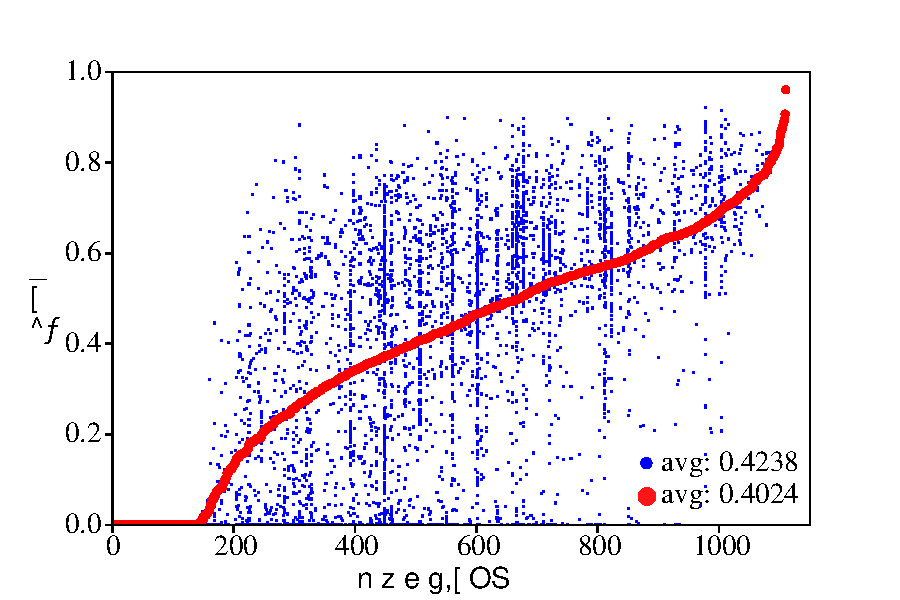
\includegraphics[width=\textwidth]{Img/fig_4_fidelity_base.pdf}
      \caption{Transformer}
      \label{fig:4_fidelity_base}
    \end{subfigure}%
    ~% add desired spacing
    \begin{subfigure}[b]{0.5\textwidth}
      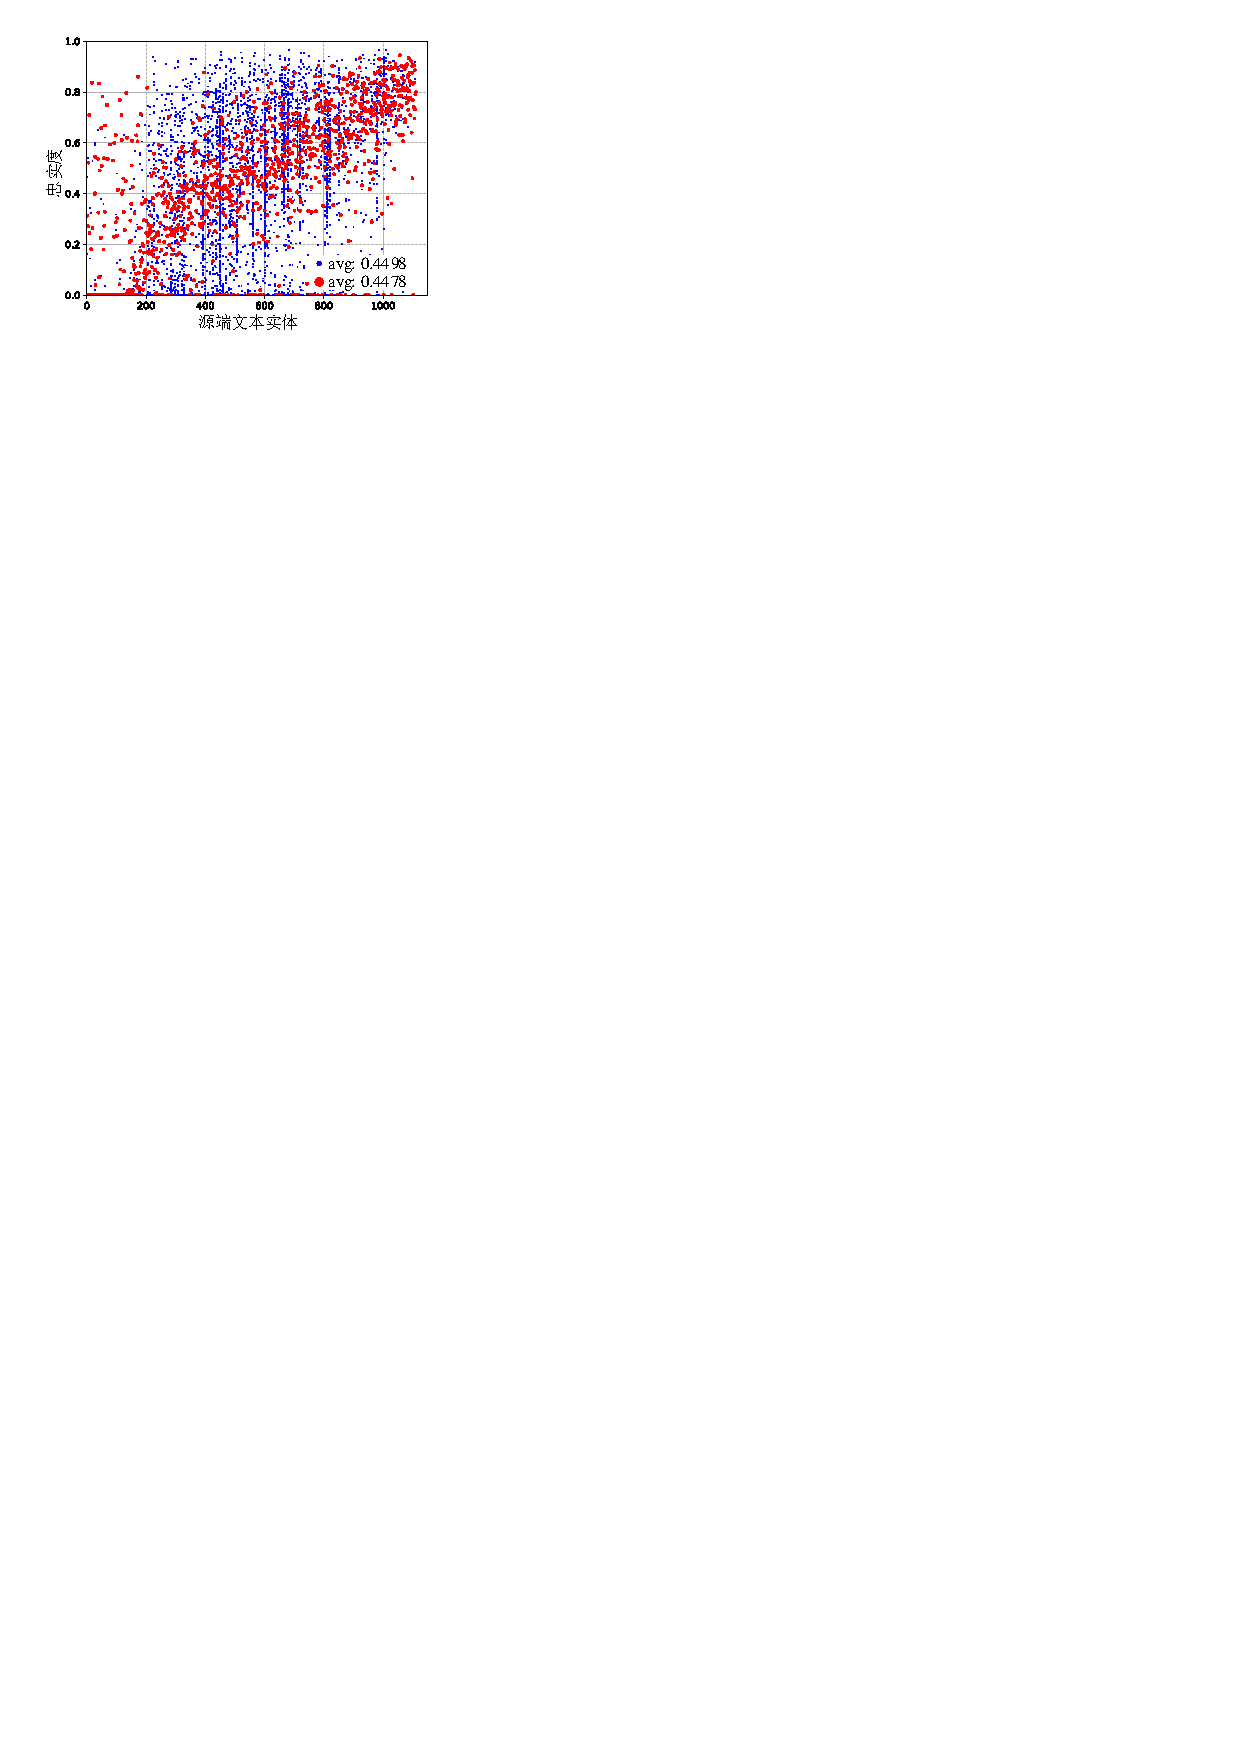
\includegraphics[width=\textwidth]{Img/fig_4_fidelity_cer_baseorder.pdf}
      \caption{CER-NMT}
      \label{fig:4_fidelity_cer_baseorder}
    \end{subfigure}
    \\% line break
    \begin{subfigure}[b]{0.5\textwidth}
      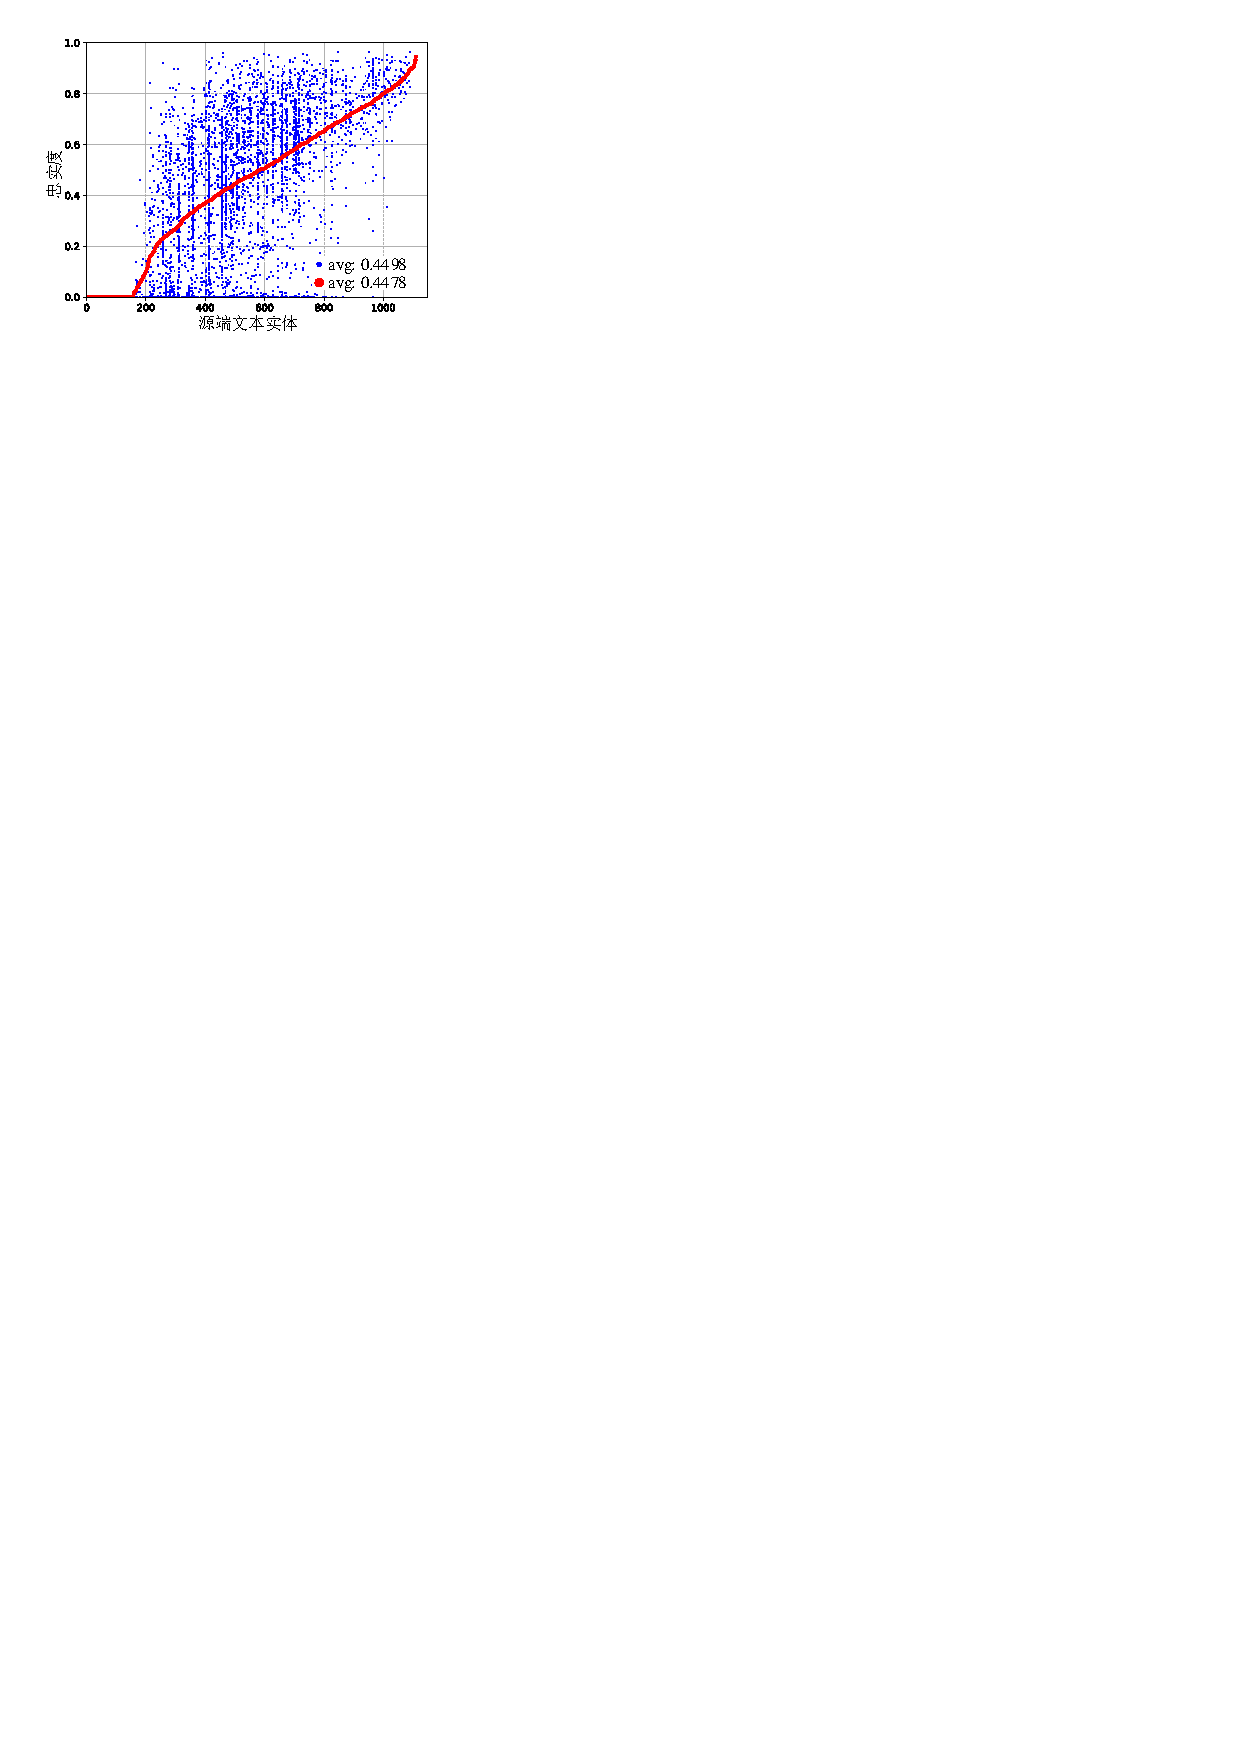
\includegraphics[width=\textwidth]{Img/fig_4_fidelity_cer_selforder.pdf}
      \caption{实体重排序的CER-NMT}
      \label{fig:4_fidelity_cer_selforder}
    \end{subfigure}%
    ~% add desired spacing
    \begin{subfigure}[b]{0.5\textwidth}
      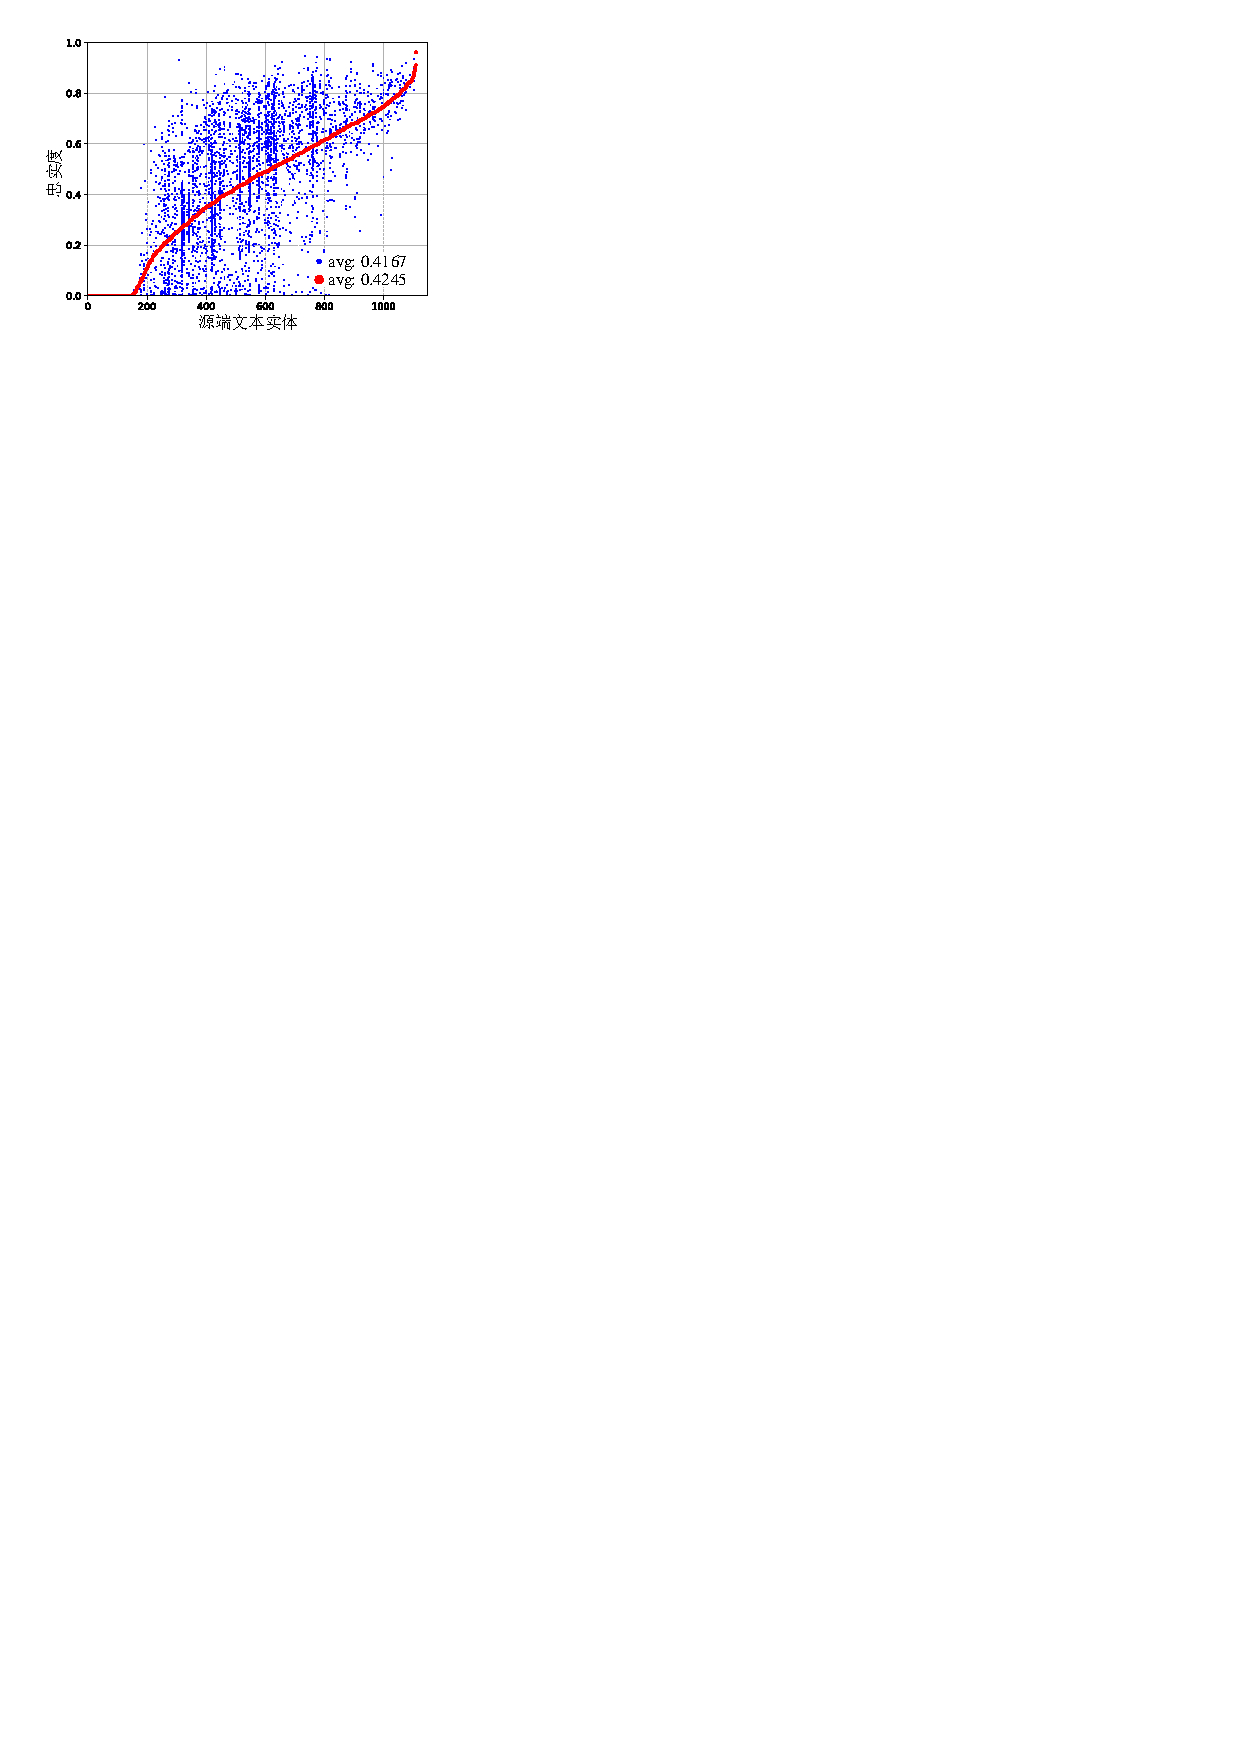
\includegraphics[width=\textwidth]{Img/fig_4_fidelity_tner.pdf}
      \caption{TNER-NMT}
      \label{fig:4_fidelity_tner}
    \end{subfigure}
    \bicaption{文本实体在不同模型下的忠实度}{The fidelity of textual entities on different models}
    \label{fig:4_fidelity}
\end{figure}
实验结果如图\ref{fig:4_fidelity}所示,图中横轴代表测试集中源语言文本实体以某种方式的排序,纵轴为范围从0到1的忠实度。每个小像素点代表一个源端文本实体在一个翻译句子样本中对应目标端文本实体的注意力权重值,即实体词忠实度。大圆点代表每个实体的平均忠实度。图\ref{fig:4_fidelity_base}为纯文本Transformer的测试结果,横轴为测试集中的1110个源端文本实体按照平均忠实度由小到大排序。图\ref{fig:4_fidelity_cer_baseorder}为CER-NMT与图\ref{fig:4_fidelity_base}横轴词序保持一致的结果,图\ref{fig:4_fidelity_cer_selforder}为CER-NMT对实体词重排序后的结果。图\ref{fig:4_fidelity_tner}为\ref{sec:4_ablation_study}节序号12仅设置TNER,且保持翻译任务训练比例不变的模型。图中“avg”代表平均值。从4个图的对比中可以得到以下信息:

%\item
(1)图中忠实度为0的横线部分代表对齐模型无法在目标端句子中找到对应的实体词。因此无法确定其忠实度。

%\item
(2)图\ref{fig:4_fidelity_cer_baseorder}相比于图\ref{fig:4_fidelity_base}存在更多靠近1.0的小像素点。从图\ref{fig:4_fidelity_cer_selforder}中的均值结果(avg)可以看到,小像素点的均值从0.4238提升至0.4498,大圆点的均值从0.4024提升至0.4478,均具有较明显的提升。该数值结果表明CER方法能够明显地提升模型在翻译过程中对源语言文本实体的忠实度。

%\item
(3)图\ref{fig:4_fidelity_cer_selforder}经过重排序实体的顺序后可以更直观地从曲线的趋势看出采用CER方法所带来的忠实度的提升。

%\item
(4)TNER对文本上下文和视觉实体进行句子级的语义融合,可以观察到图\ref{fig:4_fidelity_tner}相对于图\ref{fig:4_fidelity_base}有提升也有降低,这说明VER和TER才是帮助提升文本实体忠实度的主要因素,针对非实体的重构方法所带来的翻译性能提升无法没有显著地体现在实体忠实度的提升上。
%\end{itemize}

以上结果表明,CER方法通过融入视觉信息的方式,增加了翻译模型在翻译过程中对源语言文本实体的忠实度,从而使得翻译结果得到了进一步的提升。该实验同样表明本章的双向跨模态实体重构方法是有效可行的,该显式跨模态信息融合方法使得模型更具备可解释性,视觉信息的作用方式更有迹可循。


\section{本章小结}
本文提出了一种跨模态实体重构方法用于探究以显式方式融合视觉信息与文本信息的可行性。在翻译性能方面,实验结果表明CER$-$NMT能够在英译德和英译法两个数据集上达到更高的翻译准确率。在消融实验中发现,视觉实体重构、文本实体重构以及文本非实体重构三种重构方法组合后NMT模型从视觉信息中获益最大。最后,本文尝试验证该显式方法的可解释性,实验结果表明跨模态实体重构方法显著地增加了模型对源端文本实体的忠实度,从而带来翻译质量的提升。